\section{Fluid Properties}
        
    \begin{figure}[H]
        \centering
        % This file was created with tikzplotlib v0.10.1.
\begin{tikzpicture}

\definecolor{crimson2143940}{RGB}{214,39,40}
\definecolor{darkgray176}{RGB}{176,176,176}
\definecolor{darkorange25512714}{RGB}{255,127,14}
\definecolor{forestgreen4416044}{RGB}{44,160,44}
\definecolor{lightgray204}{RGB}{204,204,204}
\definecolor{mediumpurple148103189}{RGB}{148,103,189}
\definecolor{steelblue31119180}{RGB}{31,119,180}

\begin{groupplot}[group style={group size=1 by 3}]
\nextgroupplot[
tick align=outside,
tick pos=left,
x grid style={darkgray176},
xlabel={Temperature/K},
xmin=284.25, xmax=586.75,
xtick style={color=black},
y grid style={darkgray176},
ylabel={Enthalpy/J/kg},
ymin=-418101.349433259, ymax=681363.620649662,
ytick style={color=black}
]
\addplot [semithick, steelblue31119180, mark=*, mark size=3, mark options={solid}, only marks]
table {%
298 58.2089639
303.6122449 9831.41365
309.2244898 19727.7771
314.8367347 29749.6342
320.4489796 39898.9988
326.0612245 50177.5955
331.6734694 60586.8828
337.2857143 71128.0725
342.8979592 81802.1497
348.5102041 92609.8997
354.122449 103551.937
359.7346939 114628.731
365.3469388 125840.615
370.9591837 137187.793
376.571429 148670.336
382.183673 160288.188
387.795918 172041.178
393.408163 183929.037
399.020408 195951.408
404.632653 208107.861
410.244898 220397.9
415.857143 232820.97
421.469388 245376.458
427.081633 258063.704
432.693878 270881.999
438.306122 283830.595
443.918367 296908.708
449.530612 310115.521
455.142857 323450.189
460.755102 336911.845
466.367347 350499.598
471.979592 364212.543
477.591837 378049.758
483.204082 392010.309
488.816327 406093.253
494.428571 420297.639
500.040816 434622.511
505.653061 449066.909
511.265306 463629.87
516.877551 478310.432
522.489796 493107.631
528.102041 508020.509
533.714286 523048.106
539.326531 538189.469
544.938776 553443.648
550.55102 568809.701
556.163265 584286.688
561.77551 599873.679
567.387755 615569.75
573 631373.984
};
\addplot [semithick, steelblue31119180]
table {%
298 58.2101593370317
303.6122449 9831.63063540997
309.2244898 19728.2126500804
314.8367347 29750.2910350309
320.4489796 39899.8798416733
326.0612245 50178.7035679537
331.6734694 60588.2208642155
337.2857143 71129.6434674513
342.8979592 81803.9565777662
348.5102041 92611.9453157664
354.122449 103554.224479815
359.7346939 114631.262768611
365.3469388 125843.394937357
370.9591837 137190.823838832
376.571429 148673.621303565
382.183673 160291.728151192
387.795918 172044.978538081
393.408163 183933.100021098
399.020408 195955.736797045
404.632653 208112.458918832
410.244898 220402.770352669
415.857143 232826.114903655
421.469388 245381.8811906
427.081633 258069.407397914
432.693878 270887.986051255
438.306122 283836.866460654
443.918367 296915.268593506
449.530612 310122.373601068
455.142857 323457.337085283
460.755102 336919.290539095
466.367347 350507.34476768
471.979592 364220.593016007
477.591837 378058.113826134
483.204082 392018.973646252
488.816327 406102.229211003
494.428571 420306.927168559
500.040816 434632.116199162
505.653061 449076.833619493
511.265306 463640.117106928
516.877551 478321.003643848
522.489796 493118.530836419
528.102041 508031.738098232
533.714286 523059.667708831
539.326531 538201.365756568
544.938776 553455.882974655
550.55102 568822.27273088
556.163265 584299.602646647
561.77551 599886.938732507
567.387755 615583.356808007
573 631387.940191348
};
\addplot [semithick, darkorange25512714, mark=*, mark size=3, mark options={solid}, only marks]
table {%
298 -368117.367
303.6122449 -354337.012
309.2244898 10473.7447
314.8367347 20979.6229
320.4489796 31569.7123
326.0612245 42251.2905
331.6734694 53030.4398
337.2857143 63912.2319
342.8979592 74900.887
348.5102041 85999.9373
354.122449 97212.3866
359.7346939 108540.829
365.3469388 119987.503
370.9591837 131554.299
376.571429 143242.75
382.183673 155054.049
387.795918 166989.094
393.408163 179048.546
399.020408 191232.873
404.632653 203542.394
410.244898 215977.295
415.857143 228537.643
421.469388 241223.394
427.081633 254034.402
432.693878 266970.426
438.306122 280031.141
443.918367 293216.149
449.530612 306524.983
455.142857 319957.119
460.755102 333511.981
466.367347 347188.948
471.979592 360987.36
477.591837 374906.523
483.204082 388945.712
488.816327 403104.178
494.428571 417381.148
500.040816 431775.831
505.653061 446287.422
511.265306 460915.1
516.877551 475658.035
522.489796 490515.388
528.102041 505486.313
533.714286 520569.961
539.326531 535765.477
544.938776 551072.006
550.55102 566488.693
556.163265 582014.681
561.77551 597649.117
567.387755 613391.149
573 629239.928
};
\addplot [semithick, darkorange25512714]
table {%
298 -368125.668974945
303.6122449 -354344.998138193
309.2244898 10484.5385126809
314.8367347 20990.0277811753
320.4489796 31579.7945331162
326.0612245 42261.1067601767
331.6734694 53040.0392156682
337.2857143 63921.657408223
342.8979592 74910.1764735352
348.5102041 86009.1244572948
354.122449 97221.501484689
359.7346939 108549.898625471
365.3469388 119996.552428484
370.9591837 131563.34953266
376.571429 143251.821960464
382.183673 155063.158258236
387.795918 166998.260095048
393.408163 179057.78317317
399.020408 191242.196889367
404.632653 203551.817950731
410.244898 215986.831624928
415.857143 228547.30393775
421.469388 241233.19025531
427.081633 254044.343475284
432.693878 266980.522874712
438.306122 280041.40109141
443.918367 293226.582695844
449.530612 306535.598933739
455.142857 319967.924948704
460.755102 333522.984577836
466.367347 347200.156686695
471.979592 360998.780813674
477.591837 374918.162213264
483.204082 388957.576376827
488.816327 403116.27309565
494.428571 417393.477564512
500.040816 431788.403874896
505.653061 446300.24272224
511.265306 460928.174237987
516.877551 475671.367867084
522.489796 490528.984536982
528.102041 505500.178606629
533.714286 520584.099615216
539.326531 535779.893848576
544.938776 551086.705739511
550.55102 566503.676360063
556.163265 582029.955540582
561.77551 597664.686373282
567.387755 613407.01705272
573 629256.098906665
};
\addplot [semithick, forestgreen4416044, mark=*, mark size=3, mark options={solid}, only marks]
table {%
298 -367646.719
303.6122449 -353900.651
309.2244898 -339969.933
314.8367347 -325845.28
320.4489796 -311516.327
326.0612245 -296971.307
331.6734694 -282196.622
337.2857143 -267176.241
342.8979592 -251890.857
348.5102041 -236316.639
354.122449 72408.7622
359.7346939 85157.8483
365.3469388 97865.3772
370.9591837 110562.069
376.571429 123271.242
382.183673 136010.647
387.795918 148793.981
393.408163 161632.084
399.020408 174533.81
404.632653 187506.557
410.244898 200556.593
415.857143 213689.231
421.469388 226908.957
427.081633 240219.538
432.693878 253624.116
438.306122 267125.302
443.918367 280725.255
449.530612 294425.752
455.142857 308228.245
460.755102 322133.907
466.367347 336143.675
471.979592 350258.281
477.591837 364478.279
483.204082 378804.067
488.816327 393235.909
494.428571 407773.953
500.040816 422418.239
505.653061 437168.72
511.265306 452025.268
516.877551 466987.685
522.489796 482055.712
528.102041 497229.035
533.714286 512507.294
539.326531 527890.085
544.938776 543376.97
550.55102 558967.478
556.163265 574661.109
561.77551 590457.34
567.387755 606355.628
573 622355.409
};
\addplot [semithick, forestgreen4416044]
table {%
298 -367654.856880683
303.6122449 -353908.484908849
309.2244898 -339977.457965932
314.8367347 -325852.49246809
320.4489796 -311523.222705909
326.0612245 -296977.881519898
331.6734694 -282202.868983471
337.2857143 -267182.155698789
342.8979592 -251896.434030489
348.5102041 -236321.870954613
354.122449 72410.4219675958
359.7346939 85159.784944119
365.3469388 97867.5906216177
370.9591837 110564.559782328
376.571429 123274.011323833
382.183673 136013.693590731
387.795918 148797.307222051
393.408163 161635.6929065
399.020408 174537.701503075
404.632653 187510.734555318
410.244898 200561.057821584
415.857143 213693.984704983
421.469388 226914.002055456
427.081633 240224.875876736
432.693878 253629.749286571
438.306122 267131.230673351
443.918367 280731.483945381
449.530612 294432.283191359
455.142857 308235.080030496
460.755102 322141.048912277
466.367347 336151.12647426
471.979592 350266.044206095
477.591837 364486.355799316
483.204082 378812.460263863
488.816327 393244.621634863
494.428571 407782.983295218
500.040816 422427.592975173
505.653061 437178.39990011
511.265306 452035.276195231
516.877551 466998.023979723
522.489796 482066.383854226
528.102041 497240.042365614
533.714286 512518.638587108
539.326531 527901.769930061
544.938776 543388.997286007
550.55102 558979.846795783
556.163265 574673.825022579
561.77551 590470.405874422
567.387755 606369.044889984
573 622369.17930978
};
\addplot [semithick, crimson2143940, mark=*, mark size=3, mark options={solid}, only marks]
table {%
298 -366100.092
303.6122449 -352452.257
309.2244898 -338631.964
314.8367347 -324632.01
320.4489796 -310444.605
326.0612245 -296061.221
331.6734694 -281472.383
337.2857143 -266667.413
342.8979592 -251634.086
348.5102041 -236358.164
354.122449 -220822.76
359.7346939 -205007.435
365.3469388 -188886.874
370.9591837 -172428.884
376.571429 -155591.216
382.183673 -138316.26
387.795918 -120521.564
393.408163 -102081.366
399.020408 -82786.0735
404.632653 -62236.1033
410.244898 -39465.7068
415.857143 129504.822
421.469388 153545.174
427.081633 173891.686
432.693878 192583.634
438.306122 210330.085
443.918367 227473.289
449.530612 244208.098
455.142857 260657.389
460.755102 276904.264
466.367347 293007.844
471.979592 309011.82
477.591837 324949.44
483.204082 340846.601
488.816327 356723.853
494.428571 372597.757
500.040816 388481.823
505.653061 404387.194
511.265306 420323.138
516.877551 436297.423
522.489796 452316.599
528.102041 468386.217
533.714286 484511.002
539.326531 500694.989
544.938776 516941.632
550.55102 533253.896
556.163265 549634.323
561.77551 566085.098
567.387755 582608.097
573 599204.928
};
\addplot [semithick, crimson2143940]
table {%
298 -366108.401400303
303.6122449 -352460.253051503
309.2244898 -338639.64119466
314.8367347 -324639.361962566
320.4489796 -310451.627011864
326.0612245 -296067.905601941
331.6734694 -281478.723321133
337.2857143 -266673.401405319
342.8979592 -251639.71287421
348.5102041 -236363.419449605
354.122449 -220827.633106935
359.7346939 -205011.911816649
365.3469388 -188890.937974667
370.9591837 -172432.514141494
376.571429 -155594.385458987
382.183673 -138318.93813605
387.795918 -120523.697323517
393.408163 -102082.877237404
399.020408 -82786.8304062953
404.632653 -62235.8331172677
410.244898 -39463.6367728115
415.857143 129534.562648919
421.469388 153566.300481966
427.081633 173909.53966334
432.693878 192599.738770993
438.306122 210345.118765788
443.918367 227487.628053585
449.530612 244221.972464586
455.142857 260670.9541122
460.755102 276917.630967729
466.367347 293021.095389684
471.979592 309025.018250921
477.591837 324962.63526899
483.204082 340859.833990428
488.816327 356737.158262246
494.428571 372611.158914595
500.040816 388495.349238817
505.653061 404400.864899814
511.265306 420336.971937376
516.877551 436311.435788541
522.489796 452330.804581682
528.102041 468400.628305703
533.714286 484525.630696513
539.326531 500709.84569347
544.938776 516956.726961547
550.55102 533269.233757044
556.163265 549649.915178063
561.77551 566100.952603576
567.387755 582624.221054711
573 599221.327908611
};
\addplot [semithick, mediumpurple148103189, mark=*, mark size=3, mark options={solid}, only marks]
table {%
298 -360737.537
303.6122449 -347326.004
309.2244898 -333766.566
314.8367347 -320055.278
320.4489796 -306188.19
326.0612245 -292161.325
331.6734694 -277970.652
337.2857143 -263612.063
342.8979592 -249081.342
348.5102041 -234374.13
354.122449 -219485.892
359.7346939 -204411.877
365.3469388 -189147.068
370.9591837 -173686.134
376.571429 -158023.367
382.183673 -142152.612
387.795918 -126067.185
393.408163 -109759.766
399.020408 -93222.2883
404.632653 -76445.7863
410.244898 -59420.2278
415.857143 -42134.3102
421.469388 -24575.2333
427.081633 -6728.46437
432.693878 11422.4576
438.306122 29895.9879
443.918367 48712.3368
449.530612 67892.6262
455.142857 87456.9722
460.755102 107420.876
466.367347 127789.368
471.979592 148549.049
477.591837 169659.891
483.204082 191051.021
488.816327 212625.257
494.428571 234273.242
500.040816 255891.432
505.653061 277395.675
511.265306 298726.431
516.877551 319847.293
522.489796 340740.533
528.102041 361402.295
533.714286 381838.48
539.326531 402061.498
544.938776 422087.764
550.55102 441935.839
556.163265 461625.075
561.77551 481174.688
567.387755 500603.152
573 519927.844
};
\addplot [semithick, mediumpurple148103189]
table {%
298 -360745.532574137
303.6122449 -347333.703084717
309.2244898 -333773.964925837
314.8367347 -320062.373308075
320.4489796 -306194.978102363
326.0612245 -292167.801614804
331.6734694 -277976.814145275
337.2857143 -263617.907135885
342.8979592 -249086.863634628
348.5102041 -234379.325698596
354.122449 -219490.758227968
359.7346939 -204416.40853169
365.3469388 -189151.260649811
370.9591837 -173689.983091639
376.571429 -158026.867117108
382.183673 -142155.762703479
387.795918 -126069.977242796
393.408163 -109762.195931158
399.020408 -93224.3496623767
404.632653 -76447.4737126573
410.244898 -59421.5354109313
415.857143 -42135.2318470846
421.469388 -24575.7622916425
427.081633 -6728.59376832435
432.693878 11422.735301792
438.306122 29896.6773717169
443.918367 48713.4500195258
449.530612 67894.1724645407
455.142857 87458.9614965544
460.755102 107423.318559383
466.367347 127792.274931628
471.979592 148552.429775941
477.591837 169663.754585829
483.204082 191055.373387281
488.816327 212630.100354768
494.428571 234278.573050582
500.040816 255897.250539839
505.653061 277401.976830142
511.265306 298733.209573799
516.877551 319854.541322954
522.489796 340748.244137882
528.102041 361410.462222547
533.714286 381847.098231041
539.326531 402070.560267333
544.938776 422097.266277126
550.55102 441945.773117819
556.163265 461635.441092364
561.77551 481185.482402421
567.387755 500614.372458203
573 519939.488102578
};

\nextgroupplot[
tick align=outside,
tick pos=left,
x grid style={darkgray176},
xlabel={Temperature/K},
xmin=284.25, xmax=586.75,
xtick style={color=black},
y grid style={darkgray176},
ylabel={Entropy/J/kg},
ymin=-1527.88340261826, ymax=1605.87557596765,
ytick style={color=black}
]
\addplot [semithick, steelblue31119180, mark=*, mark size=3, mark options={solid}, only marks]
table {%
298 2.02197728
303.6122449 34.5123356
309.2244898 66.8095192
314.8367347 98.9279625
320.4489796 130.880325
326.0612245 162.677709
331.6734694 194.329843
337.2857143 225.845224
342.8979592 257.231264
348.5102041 288.494436
354.122449 319.640415
359.7346939 350.674201
365.3469388 381.600191
370.9591837 412.422225
376.571429 443.143613
382.183673 473.767189
387.795918 504.29536
393.408163 534.730178
399.020408 565.073388
404.632653 595.32648
410.244898 625.490719
415.857143 655.567174
421.469388 685.556739
427.081633 715.460151
432.693878 745.278016
438.306122 775.01082
443.918367 804.658948
449.530612 834.2227
455.142857 863.702304
460.755102 893.097925
466.367347 922.40968
471.979592 951.637641
477.591837 980.781849
483.204082 1009.84232
488.816327 1038.81904
494.428571 1067.712
500.040816 1096.52115
505.653061 1125.24647
511.265306 1153.8879
516.877551 1182.44541
522.489796 1210.91896
528.102041 1239.30852
533.714286 1267.61405
539.326531 1295.83553
544.938776 1323.97296
550.55102 1352.02633
556.163265 1379.99566
561.77551 1407.88096
567.387755 1435.68227
573 1463.39964
};
\addplot [semithick, steelblue31119180]
table {%
298 2.0220217688493
303.6122449 34.51309744523
309.2244898 66.8109943019645
314.8367347 98.9301469925199
320.4489796 130.883214824198
326.0612245 162.681301715266
331.6734694 194.33413450506
337.2857143 225.850212013348
342.8979592 257.236946011631
348.5102041 288.500808335818
354.122449 319.647475668181
359.7346939 350.681947462985
365.3469388 381.608621466479
370.9591837 412.431335979245
376.571429 443.153405791052
382.183673 473.777653238104
387.795918 504.3065000723
393.408163 534.741990621663
399.020408 565.085871929474
404.632653 595.339633274502
410.244898 625.504540159306
415.857143 655.581660824491
421.469388 685.571888711707
427.081633 715.47596291412
432.693878 745.294487346931
438.306122 775.027943360948
443.918367 804.676727364378
449.530612 834.24113388659
455.142857 863.721390031152
460.755102 893.117661895208
466.367347 922.430064905506
471.979592 951.658672910145
477.591837 980.803526163611
483.204082 1009.86463832852
488.816327 1038.84200260236
494.428571 1067.73559192348
500.040816 1096.54538420017
505.653061 1125.27133544975
511.265306 1153.91340388085
516.877551 1182.47154771642
522.489796 1210.94572773109
528.102041 1239.33590939579
533.714286 1267.64206467322
539.326531 1295.86417350387
544.938776 1324.00222501801
550.55102 1352.05621351474
556.163265 1380.0261591991
561.77551 1407.91207876025
567.387755 1435.71400578818
573 1463.43198603193
};
\addplot [semithick, darkorange25512714, mark=*, mark size=3, mark options={solid}, only marks]
table {%
298 -1354.22791
303.6122449 -1308.41611
309.2244898 -119.459598
314.8367347 -85.789692
320.4489796 -52.4496215
326.0612245 -19.4054116
331.6734694 13.3715375
337.2857143 45.9053633
342.8979592 78.2165033
348.5102041 110.322409
354.122449 142.23819
359.7346939 173.977095
365.3469388 205.55078
370.9591837 236.969414
376.571429 268.241757
382.183673 299.375287
387.795918 330.376384
393.408163 361.250543
399.020408 392.002548
404.632653 422.636601
410.244898 453.156411
415.857143 483.565243
421.469388 513.865969
427.081633 544.061104
432.693878 574.152846
438.306122 604.143116
443.918367 634.033591
449.530612 663.825733
455.142857 693.520826
460.755102 723.119989
466.367347 752.624207
471.979592 782.034344
477.591837 811.351161
483.204082 840.575333
488.816327 869.707455
494.428571 898.748058
500.040816 927.697619
505.653061 956.556566
511.265306 985.325286
516.877551 1014.00413
522.489796 1042.59344
528.102041 1071.0935
533.714286 1099.50461
539.326531 1127.82703
544.938776 1156.06103
550.55102 1184.20685
556.163265 1212.26473
561.77551 1240.23491
567.387755 1268.11763
573 1295.91313
};
\addplot [semithick, darkorange25512714]
table {%
298 -1354.25726403103
303.6122449 -1308.44442068368
309.2244898 -119.334119527088
314.8367347 -85.6654605660792
320.4489796 -52.3264062670955
326.0612245 -19.2830193535756
331.6734694 13.4932701946395
337.2857143 46.0265757766629
342.8979592 78.3373155995669
348.5102041 110.442925001832
354.122449 142.358500273288
359.7346939 174.097279063133
365.3469388 205.670906156791
370.9591837 237.089543253642
376.571429 268.361945407788
382.183673 299.495573610484
387.795918 330.496817129798
393.408163 361.37115982476
399.020408 392.123382166441
404.632653 422.757684212001
410.244898 453.277769781966
415.857143 483.686902982175
421.469388 513.987952288242
427.081633 544.183430787104
432.693878 574.275535318316
438.306122 604.26617884317
443.918367 634.157046929423
449.530612 663.949597413536
455.142857 693.64510984759
460.755102 723.244704681464
466.367347 752.749364636576
471.979592 782.159953328906
477.591837 811.477231524926
483.204082 840.701871360076
488.816327 869.834468794255
494.428571 898.875549365823
500.040816 927.825598450264
505.653061 956.685038608014
511.265306 985.454257652954
516.877551 1014.13360990396
522.489796 1042.72342180619
528.102041 1071.22399683313
533.714286 1099.63561975238
539.326531 1127.95856032834
544.938776 1156.19307652687
550.55102 1184.33941227223
556.163265 1212.39781986718
561.77551 1240.36853193357
567.387755 1268.25178321715
573 1296.04780702596
};
\addplot [semithick, forestgreen4416044, mark=*, mark size=3, mark options={solid}, only marks]
table {%
298 -1356.64782
303.6122449 -1310.94999
309.2244898 -1265.48659
314.8367347 -1220.21945
320.4489796 -1175.10898
326.0612245 -1130.11336
331.6734694 -1085.18733
337.2857143 -1040.28062
342.8979592 -995.335844
348.5102041 -950.285317
354.122449 -74.5939288
359.7346939 -38.874101
365.3469388 -3.82200774
370.9591837 30.6661896
376.571429 64.6698372
382.183673 98.2500826
387.795918 131.454857
393.408163 164.322717
399.020408 196.885554
404.632653 229.170311
410.244898 261.200033
415.857143 292.994516
421.469388 324.570787
427.081633 355.943497
432.693878 387.125275
438.306122 418.127038
443.918367 448.958264
449.530612 479.627214
455.142857 510.141126
460.755102 540.506365
466.367347 570.728552
471.979592 600.812669
477.591837 630.763147
483.204082 660.583939
488.816327 690.278585
494.428571 719.850262
500.040816 749.30183
505.653061 778.635877
511.265306 807.854744
516.877551 836.960562
522.489796 865.955274
528.102041 894.840657
533.714286 923.618343
539.326531 952.289836
544.938776 980.856522
550.55102 1009.31969
556.163265 1037.68054
561.77551 1065.94019
567.387755 1094.09969
573 1122.16001
};
\addplot [semithick, forestgreen4416044]
table {%
298 -1356.6780373682
303.6122449 -1310.97919884115
309.2244898 -1265.51479713853
314.8367347 -1220.24664834478
320.4489796 -1175.13518691756
326.0612245 -1130.13857410789
331.6734694 -1085.21154206434
337.2857143 -1040.30384068219
342.8979592 -995.358071820802
348.5102041 -950.306547569198
354.122449 -74.5954518371254
359.7346939 -38.8748482416254
365.3469388 -3.8219915513273
370.9591837 30.6669584861534
376.571429 64.6713519424566
382.183673 98.2523271491214
387.795918 131.457829483158
393.408163 164.326411790089
399.020408 196.889964030137
404.632653 229.175431598293
410.244898 261.205857873283
415.857143 293.001040672964
421.469388 324.578006895812
427.081633 355.951408338975
432.693878 387.133873643674
438.306122 418.136315089892
443.918367 448.968220515519
449.530612 479.637847300048
455.142857 510.152432430959
460.755102 540.518341439903
466.367347 570.741195532661
471.979592 600.825976843338
477.591837 630.777116270945
483.204082 660.59856737028
488.816327 690.293868958478
494.428571 719.866193224497
500.040816 749.318412505787
505.653061 778.65310700823
511.265306 807.872619863894
516.877551 836.979081258748
522.489796 865.974433966588
528.102041 894.860455571602
533.714286 923.638777849657
539.326531 952.310903703531
544.938776 980.878221985901
550.55102 1009.34201543085
556.163265 1037.70349232877
561.77551 1065.9637661215
567.387755 1094.12388452844
573 1122.18483223475
};
\addplot [semithick, crimson2143940, mark=*, mark size=3, mark options={solid}, only marks]
table {%
298 -1364.05209
303.6122449 -1318.68078
309.2244898 -1273.57771
314.8367347 -1228.71013
320.4489796 -1184.04521
326.0612245 -1139.54953
331.6734694 -1095.18851
337.2857143 -1050.9257
342.8979592 -1006.72192
348.5102041 -962.534071
354.122449 -918.313593
359.7346939 -874.004255
365.3469388 -829.538999
370.9591837 -784.835156
376.571429 -739.786893
382.183673 -694.252602
387.795918 -648.032374
393.408163 -600.824114
399.020408 -552.127156
404.632653 -500.989464
410.244898 -445.11069
415.857143 -36.8430746
421.469388 20.5951013
427.081633 68.5575233
432.693878 112.042167
438.306122 152.794148
443.918367 191.659433
449.530612 229.121856
455.142857 265.488012
460.755102 300.966313
466.367347 335.70584
471.979592 369.817419
477.591837 403.385945
483.204082 436.47803
488.816327 469.146973
494.428571 501.436126
500.040816 533.381241
505.653061 565.012162
511.265306 596.354056
516.877551 627.428348
522.489796 658.253423
528.102041 688.845178
533.714286 719.217445
539.326531 749.382339
544.938776 779.350528
550.55102 809.131451
556.163265 838.733506
561.77551 868.164194
567.387755 897.430245
573 926.537719
};
\addplot [semithick, crimson2143940]
table {%
298 -1364.08153671443
303.6122449 -1318.7091840065
309.2244898 -1273.60506782036
314.8367347 -1228.73645182068
320.4489796 -1184.07049548305
326.0612245 -1139.57377290471
331.6734694 -1095.21170089496
337.2857143 -1050.94783749905
342.8979592 -1006.74299390837
348.5102041 -962.554073744887
354.122449 -918.332506107832
359.7346939 -874.022057452923
365.3469388 -829.555662360951
370.9591837 -784.850642556424
376.571429 -739.801147659964
382.183673 -694.265560394495
387.795918 -648.043917557097
393.408163 -600.834066194938
399.020408 -552.135203995691
404.632653 -500.994956621508
410.244898 -445.111768935709
415.857143 -36.7728203552597
421.469388 20.6447513717258
427.081633 68.5994518123002
432.693878 112.080025492123
438.306122 152.829545397738
443.918367 191.693254515388
449.530612 229.154638946485
455.142857 265.520111640164
460.755102 300.997979010096
466.367347 335.737254972793
471.979592 369.848720860376
477.591837 403.417241500254
483.204082 436.509405524382
488.816327 469.178495840959
494.428571 501.467845836105
500.040816 533.413210848272
505.653061 565.044419332958
511.265306 596.386634042185
516.877551 627.461273817599
522.489796 658.286720612972
528.102041 688.878866629483
533.714286 719.251543441381
539.326531 749.416862619144
544.938776 779.385489024145
550.55102 809.166856929349
556.163265 838.769372172404
561.77551 868.200529406638
567.387755 897.467057087709
573 926.575015524127
};
\addplot [semithick, mediumpurple148103189, mark=*, mark size=3, mark options={solid}, only marks]
table {%
298 -1385.40899
303.6122449 -1340.82315
309.2244898 -1296.57127
314.8367347 -1252.6287
320.4489796 -1208.97207
326.0612245 -1165.57915
331.6734694 -1122.42868
337.2857143 -1079.50023
342.8979592 -1036.77409
348.5102041 -994.231081
354.122449 -951.852437
359.7346939 -909.619675
365.3469388 -867.514445
370.9591837 -825.518377
376.571429 -783.612922
382.183673 -741.779178
387.795918 -699.997688
393.408163 -658.248217
399.020408 -616.509495
404.632653 -574.758915
410.244898 -532.972181
415.857143 -491.122916
421.469388 -449.182224
427.081633 -407.118275
432.693878 -364.895999
438.306122 -322.477104
443.918367 -279.820777
449.530612 -236.885702
455.142857 -193.634316
460.755102 -150.040508
466.367347 -106.101683
471.979592 -61.8546095
477.591837 -17.3908213
483.204082 27.1371449
488.816327 71.5278816
494.428571 115.562083
500.040816 159.039521
505.653061 201.805228
511.265306 243.757765
516.877551 284.844027
522.489796 325.048583
528.102041 364.382913
533.714286 402.87652
539.326531 440.570111
544.938776 477.510529
550.55102 513.747092
556.163265 549.329051
561.77551 584.303929
567.387755 618.71652
573 652.608372
};
\addplot [semithick, mediumpurple148103189]
table {%
298 -1385.43981268254
303.6122449 -1340.8529819698
309.2244898 -1296.60012406397
314.8367347 -1252.65658079035
320.4489796 -1208.99898441411
326.0612245 -1165.60509926019
331.6734694 -1122.45367010798
337.2857143 -1079.52427610158
342.8979592 -1036.79718882171
348.5102041 -994.253233027365
354.122449 -951.873648363623
359.7346939 -909.639949986941
365.3469388 -867.533785516795
370.9591837 -825.536785015521
376.571429 -783.630396953112
382.183673 -741.795730096843
387.795918 -700.013310321606
393.408163 -658.262910367632
399.020408 -616.523259015132
404.632653 -574.771747829935
410.244898 -532.984081940759
415.857143 -491.133881996735
421.469388 -449.19225237101
427.081633 -407.127361708713
432.693878 -364.904139260451
438.306122 -322.484298327056
443.918367 -279.827010791671
449.530612 -236.890965957018
455.142857 -193.638600899736
460.755102 -150.043802024245
466.367347 -106.103976119015
471.979592 -61.8558926064043
477.591837 -17.391087990512
483.204082 27.1378953946009
488.816327 71.5296434384572
494.428571 115.564836264362
500.040816 159.043255924105
505.653061 201.809922624562
511.265306 243.763396758053
516.877551 284.850572753333
522.489796 325.056019752627
528.102041 364.391218599767
533.714286 402.88567360112
539.326531 440.580093560801
544.938776 477.52132314857
550.55102 513.758674690837
556.163265 549.341413766281
561.77551 584.31705812003
567.387755 618.730404056196
573 652.622998746794
};

\nextgroupplot[
legend cell align={left},
legend style={
  fill opacity=0.8,
  draw opacity=1,
  text opacity=1,
  at={(0.97,0.03)},
  anchor=south east,
  draw=lightgray204
},
tick align=outside,
tick pos=left,
unbounded coords=jump,
x grid style={darkgray176},
xlabel={Temperature/K},
xmin=284.25, xmax=586.75,
xtick style={color=black},
y grid style={darkgray176},
ylabel={Density/kg/m3},
ymin=-28.1158954066006, ymax=617.354055209838,
ytick style={color=black}
]
\addplot [semithick, black, mark=*, mark size=3, mark options={solid}, only marks]
table {%
nan nan
nan nan
};
\addlegendentry{AspenPlus}
\addplot [semithick, black]
table {%
nan nan
nan nan
};
\addlegendentry{PowerCycle}
\addplot [semithick, steelblue31119180]
table {%
nan nan
nan nan
};
\addlegendentry{\qty{1.00}{\bar}}
\addplot [semithick, darkorange25512714]
table {%
nan nan
nan nan
};
\addlegendentry{\qty{3.16}{\bar}}
\addplot [semithick, forestgreen4416044]
table {%
nan nan
nan nan
};
\addlegendentry{\qty{10.00}{\bar}}
\addplot [semithick, crimson2143940]
table {%
nan nan
nan nan
};
\addlegendentry{\qty{31.62}{\bar}}
\addplot [semithick, mediumpurple148103189]
table {%
nan nan
nan nan
};
\addlegendentry{\qty{100.00}{\bar}}
\addplot [semithick, steelblue31119180, mark=*, mark size=3, mark options={solid}, only marks, forget plot]
table {%
298 2.41764881
303.6122449 2.36842732
309.2244898 2.32137809
314.8367347 2.27634256
320.4489796 2.23317899
326.0612245 2.1917601
331.6734694 2.15197117
337.2857143 2.11370831
342.8979592 2.07687718
348.5102041 2.04139176
354.122449 2.00717341
359.7346939 1.97415007
365.3469388 1.94225547
370.9591837 1.91142859
376.571429 1.8816131
382.183673 1.85275684
387.795918 1.82481146
393.408163 1.797732
399.020408 1.77147663
404.632653 1.74600631
410.244898 1.72128459
415.857143 1.69727736
421.469388 1.67395268
427.081633 1.65128059
432.693878 1.62923293
438.306122 1.60778324
443.918367 1.58690659
449.530612 1.56657949
455.142857 1.54677976
460.755102 1.52748646
466.367347 1.50867979
471.979592 1.490341
477.591837 1.47245233
483.204082 1.45499694
488.816327 1.43795885
494.428571 1.42132288
500.040816 1.40507461
505.653061 1.3892003
511.265306 1.3736869
516.877551 1.35852196
522.489796 1.34369362
528.102041 1.32919054
533.714286 1.31500195
539.326531 1.30111751
544.938776 1.28752736
550.55102 1.27422208
556.163265 1.26119265
561.77551 1.24843043
567.387755 1.23592714
573 1.22367487
};
\addplot [semithick, steelblue31119180, forget plot]
table {%
298 2.41759523306978
303.6122449 2.36837484229437
309.2244898 2.32132666612581
314.8367347 2.27629213780953
320.4489796 2.23312952393764
326.0612245 2.19171156356317
331.6734694 2.15192351218479
337.2857143 2.11366150688394
342.8979592 2.07683119170406
348.5102041 2.04134655993771
354.122449 2.0071289789217
359.7346939 1.97410636441517
365.3469388 1.94221247235461
370.9591837 1.91138628135877
376.571429 1.88157144682204
382.183673 1.8527158350404
387.795918 1.82477107260697
393.408163 1.79769221944105
399.020408 1.7714374286091
404.632653 1.74596767282588
410.244898 1.72124649785262
415.857143 1.69723980262077
421.469388 1.67391564218574
427.081633 1.65124405065448
432.693878 1.62919688182276
438.306122 1.6077476693448
443.918367 1.58687148196816
449.530612 1.56654482931241
455.142857 1.5467455403653
460.755102 1.52745267103039
466.367347 1.50864641650197
471.979592 1.49030803139449
477.591837 1.47241975680013
483.204082 1.45496475355276
488.816327 1.43792704106485
494.428571 1.4212914441093
500.040816 1.40504352941125
505.653061 1.38916957589403
511.265306 1.37365651892028
516.877551 1.35849191281569
522.489796 1.34366389344387
528.102041 1.32916114355811
533.714286 1.31497286068426
539.326531 1.30108872731466
544.938776 1.28749888321503
550.55102 1.27419390201211
556.163265 1.26116475777757
561.77551 1.24840281689434
567.387755 1.23589980766694
573 1.22364780323751
};
\addplot [semithick, darkorange25512714, mark=*, mark size=3, mark options={solid}, only marks, forget plot]
table {%
298 573.149716
303.6122449 566.494411
309.2244898 7.84118574
314.8367347 7.65334331
320.4489796 7.47685879
326.0612245 7.31049937
331.6734694 7.15322722
337.2857143 7.00415982
342.8979592 6.86253985
348.5102041 6.7277121
354.122449 6.59910567
359.7346939 6.47622009
365.3469388 6.35861418
370.9591837 6.24589709
376.571429 6.13772069
382.183673 6.03377338
387.795918 5.93377489
393.408163 5.83747202
399.020408 5.74463521
404.632653 5.65505563
410.244898 5.56854274
415.857143 5.48492219
421.469388 5.40403403
427.081633 5.32573116
432.693878 5.24987795
438.306122 5.17634905
443.918367 5.10502837
449.530612 5.03580816
455.142857 4.96858823
460.755102 4.90327524
466.367347 4.83978208
471.979592 4.77802732
477.591837 4.71793473
483.204082 4.65943282
488.816327 4.60245449
494.428571 4.54693663
500.040816 4.49281984
505.653061 4.44004813
511.265306 4.38856865
516.877551 4.33833151
522.489796 4.28928949
528.102041 4.2413979
533.714286 4.1946144
539.326531 4.14889882
544.938776 4.10421304
550.55102 4.06052081
556.163265 4.01778769
561.77551 3.97598088
567.387755 3.93506914
573 3.89502271
};
\addplot [semithick, darkorange25512714, forget plot]
table {%
298 573.137486019884
303.6122449 566.482289415752
309.2244898 7.83475910671782
314.8367347 7.6471171323503
320.4489796 7.47081633082805
326.0612245 7.30462626577755
331.6734694 7.14751101859409
337.2857143 6.99858963399849
342.8979592 6.85710608615746
348.5102041 6.72240625371857
354.122449 6.59392015245148
359.7346939 6.47114807027825
365.3469388 6.35364951743245
370.9591837 6.24103419514934
376.571429 6.1329544824283
382.183673 6.02909923514363
387.795918 5.92918851417772
393.408163 5.83296949384823
399.020408 5.74021290954512
404.632653 5.65071019282007
410.244898 5.56427103747098
415.857143 5.48072131603352
421.469388 5.39990127977106
427.081633 5.32166399637893
432.693878 5.24587399112632
438.306122 5.17240607601842
443.918367 5.10114426461944
449.530612 5.03198094624828
455.142857 4.96481603915612
460.755102 4.89955630410545
466.367347 4.83611472562893
471.979592 4.77440996304
477.591837 4.71436586177834
483.204082 4.655911017159
488.816327 4.59897838381251
494.428571 4.54350493486339
500.040816 4.48943130717377
505.653061 4.43670157606167
511.265306 4.38526295824098
516.877551 4.3350655887313
522.489796 4.28606230921739
528.102041 4.23820847551131
533.714286 4.19146178205825
539.326531 4.14578210168315
544.938776 4.10113133899655
550.55102 4.05747330376051
556.163265 4.01477355666324
561.77551 3.97299934265243
567.387755 3.93211945531105
573 3.89210414852525
};
\addplot [semithick, forestgreen4416044, mark=*, mark size=3, mark options={solid}, only marks, forget plot]
table {%
298 574.326876
303.6122449 567.756883
309.2244898 561.032746
314.8367347 554.137265
320.4489796 547.050431
326.0612245 539.748699
331.6734694 532.203996
337.2857143 524.382331
342.8979592 516.24181
348.5102041 507.729681
354.122449 24.6133033
359.7346939 23.8394086
365.3469388 23.1388787
370.9591837 22.4991498
376.571429 21.9106915
382.183673 21.366087
387.795918 20.8594368
393.408163 20.3859627
399.020408 19.9417382
404.632653 19.5234974
410.244898 19.1284961
415.857143 18.7544074
421.469388 18.3992417
427.081633 18.0612843
432.693878 17.7390467
438.306122 17.4312282
443.918367 17.136685
449.530612 16.8544057
455.142857 16.5834915
460.755102 16.3231396
466.367347 16.0726301
471.979592 15.8313147
477.591837 15.5986075
483.204082 15.373977
488.816327 15.1569397
494.428571 14.9470543
500.040816 14.7439169
505.653061 14.5471569
511.265306 14.3564332
516.877551 14.1714315
522.489796 13.991861
528.102041 13.8174527
533.714286 13.6479568
539.326531 13.483141
544.938776 13.322789
550.55102 13.1666988
556.163265 13.014682
561.77551 12.8665618
567.387755 12.7221729
573 12.5813597
};
\addplot [semithick, forestgreen4416044, forget plot]
table {%
298 574.315016540289
303.6122449 567.745158061198
309.2244898 561.02115998696
314.8367347 554.125821220691
320.4489796 547.039133182523
326.0612245 539.737551685277
331.6734694 532.193003764061
337.2857143 524.371500677226
342.8979592 516.231147344181
348.5102041 507.719192746966
354.122449 24.6127476522673
359.7346939 23.8388715406736
365.3469388 23.138358404718
370.9591837 22.498644557806
376.571429 21.9102001029586
382.183673 21.3656084763373
387.795918 20.8589700091312
393.408163 20.3855069203169
399.020408 19.9412926767992
404.632653 19.5230614908687
410.244898 19.1280692651762
415.857143 18.7539891707444
421.469388 18.3988315857262
427.081633 18.0608818823109
432.693878 17.7386516456479
438.306122 17.4308401926486
443.918367 17.1363036827629
449.530612 16.8540308303513
455.142857 16.5831227537939
460.755102 16.3227767551005
466.367347 16.0722729142724
471.979592 15.8309629611403
477.591837 15.5982609709194
483.204082 15.3736355331384
488.816327 15.1566031206567
494.428571 14.9467224802486
500.040816 14.7435896516871
505.653061 14.5468340357412
511.265306 14.3561146525869
516.877551 14.1711170643055
522.489796 13.9915506608594
528.102041 13.8171462868258
533.714286 13.6476541586262
539.326531 13.4828420304404
544.938776 13.3224935738667
550.55102 13.1664069694353
556.163265 13.0143935198716
561.77551 12.8662766793994
567.387755 12.7218909251953
573 12.5810808747486
};
\addplot [semithick, crimson2143940, mark=*, mark size=3, mark options={solid}, only marks, forget plot]
table {%
298 577.903092
303.6122449 571.579118
309.2244898 565.128509
314.8367347 558.538784
320.4489796 551.795808
326.0612245 544.883441
331.6734694 537.783098
337.2857143 530.473159
342.8979592 522.928196
348.5102041 515.117908
354.122449 507.005658
359.7346939 498.546376
365.3469388 489.683481
370.9591837 480.344198
376.571429 470.432113
382.183673 459.814687
387.795918 448.300881
393.408163 435.597408
399.020408 421.212318
404.632653 404.201353
410.244898 382.265339
415.857143 102.12699
421.469388 91.3295671
427.081633 84.4951857
432.693878 79.4343299
438.306122 75.4061329
443.918367 72.0603811
449.530612 69.2013139
455.142857 66.7075948
460.755102 64.4985127
466.367347 62.5175391
471.979592 60.723491
477.591837 59.0854146
483.204082 57.5794464
488.816327 56.1867975
494.428571 54.892408
500.040816 53.6840212
505.653061 52.5515287
511.265306 51.486496
516.877551 50.4818129
522.489796 49.5314301
528.102041 48.6301587
533.714286 47.7735144
539.326531 46.957596
544.938776 46.1789884
550.55102 45.4346852
556.163265 44.7220267
561.77551 44.0386478
567.387755 43.3824369
573 42.7515006
};
\addplot [semithick, crimson2143940, forget plot]
table {%
298 577.890707731082
303.6122449 571.566833694212
309.2244898 565.116324809892
314.8367347 558.526699470066
320.4489796 551.783820912029
326.0612245 544.871550679351
331.6734694 537.771302038764
337.2857143 530.461455416537
342.8979592 522.91657972788
348.5102041 515.106374514022
354.122449 506.994200280862
359.7346939 498.534983579606
365.3469388 489.672139745213
370.9591837 480.332888063005
376.571429 470.420803443514
382.183673 459.803334744577
387.795918 448.289412369724
393.408163 435.585696370021
399.020408 421.200124679918
404.632653 404.188140040775
410.244898 382.249447478983
415.857143 102.094968938083
421.469388 91.3081229120629
427.081633 84.4780272022219
432.693878 79.4196417798015
438.306122 75.3931003728451
443.918367 72.0485554713522
449.530612 69.1904180718015
455.142857 66.6974434805131
460.755102 64.4889747176103
466.367347 62.5085177345159
471.979592 60.7149126379217
477.591837 59.077221563959
483.204082 57.5715926636604
488.816327 56.1792454308712
494.428571 54.8851267823771
500.040816 53.6769846232637
505.653061 52.5447146415024
511.265306 51.4798856180904
516.877551 50.4753898399332
522.489796 49.525180184081
528.102041 48.6240694032253
533.714286 47.7675747387177
539.326531 46.9517961022758
544.938776 46.1733194819328
550.55102 45.4291396828139
556.163265 44.7165972124299
561.77551 44.0333280135563
567.387755 43.3772209380065
573 42.7463830967787
};
\addplot [semithick, mediumpurple148103189, mark=*, mark size=3, mark options={solid}, only marks, forget plot]
table {%
298 588.014512
303.6122449 582.295403
309.2244898 576.504568
314.8367347 570.636789
320.4489796 564.686507
326.0612245 558.647787
331.6734694 552.514277
337.2857143 546.279175
342.8979592 539.935178
348.5102041 533.47443
354.122449 526.888472
359.7346939 520.16817
365.3469388 513.303651
370.9591837 506.284215
376.571429 499.09825
382.183673 491.733117
387.795918 484.175033
393.408163 476.408925
399.020408 468.418264
404.632653 460.184873
410.244898 451.688712
415.857143 442.907644
421.469388 433.817202
427.081633 424.390409
432.693878 414.59775
438.306122 404.407504
443.918367 393.786789
449.530612 382.703954
455.142857 371.133215
460.755102 359.062687
466.367347 346.506657
471.979592 333.521283
477.591837 320.219184
483.204082 306.773884
488.816327 293.404917
494.428571 280.343793
500.040816 267.794808
505.653061 255.90837
511.265306 244.774001
516.877551 234.427981
522.489796 224.866776
528.102041 216.060258
533.714286 207.962349
539.326531 200.518825
544.938776 193.672694
550.55102 187.367714
556.163265 181.550521
561.77551 176.171783
567.387755 171.186682
573 166.554984
};
\addplot [semithick, mediumpurple148103189, forget plot]
table {%
298 588.002351623943
303.6122449 582.283360145531
309.2244898 576.492643129229
314.8367347 570.624984294489
320.4489796 564.674824075907
326.0612245 558.636226419791
331.6734694 552.502841959
337.2857143 546.267867107279
342.8979592 539.923998537159
348.5102041 533.463382414757
354.122449 526.877557652902
359.7346939 520.157392292869
365.3469388 513.293011890052
370.9591837 506.273718419396
376.571429 499.087897189249
382.183673 491.722913529498
387.795918 484.164981317452
393.408163 476.399028962487
399.020408 468.408527414706
404.632653 460.175300201485
410.244898 451.679307640101
415.857143 442.898412837396
421.469388 433.808149594313
427.081633 424.381541039448
432.693878 414.589072759432
438.306122 404.399024202581
443.918367 393.77851262547
449.530612 382.695888662435
455.142857 371.125367407952
460.755102 359.055064376816
466.367347 346.499266956851
471.979592 333.51413202538
477.591837 320.212278391718
483.204082 306.767229063145
488.816327 293.39851451344
494.428571 280.3376438227
500.040816 267.788906199654
505.653061 255.902706568558
511.265306 244.768566604489
516.877551 234.422762660852
522.489796 224.861760770499
528.102041 216.055431977753
533.714286 207.957699664853
539.326531 200.514338896365
544.938776 193.668359825352
550.55102 187.363521782127
556.163265 181.546459831811
561.77551 176.167842391537
567.387755 171.182854301901
573 166.551261193286
};
\end{groupplot}

\end{tikzpicture}

        \caption{Comparing properties of n-Butane as calculated by Aspen Plus v11 and PowerCycle (using CoolProp)}
        \label{fig:powercycle_val_butane}
    \end{figure}
    
    \begin{figure}[H]
        \centering
        % This file was created with tikzplotlib v0.10.1.
\begin{tikzpicture}

\definecolor{crimson2143940}{RGB}{214,39,40}
\definecolor{darkgray176}{RGB}{176,176,176}
\definecolor{darkorange25512714}{RGB}{255,127,14}
\definecolor{forestgreen4416044}{RGB}{44,160,44}
\definecolor{lightgray204}{RGB}{204,204,204}
\definecolor{mediumpurple148103189}{RGB}{148,103,189}
\definecolor{steelblue31119180}{RGB}{31,119,180}

\begin{groupplot}[
    group style={
        group size=2 by 2,
        vertical sep=2cm,
        horizontal sep=2.5cm
        },
    width=7cm,
    height=6.5cm,
    legend style={
        at={(1.65,0.5)},
        anchor=west
        },
    legend cell align={left},
    unbounded coords=jump,
    xlabel={Temperature/\unit{\K}},
    ylabel near ticks,
    xlabel near ticks,
    xmin=299, xmax=573,
    ]
\nextgroupplot[
ylabel={Enthalpy/\unit{\joule\per\kg}},
]
\addplot [semithick, steelblue31119180, mark=x, mark size=3, mark options={solid}, only marks]
table {%
298 -1.10754519
303.6122449 13066.9711
309.2244898 384045.262
314.8367347 393967.016
320.4489796 404010.846
326.0612245 414178.592
331.6734694 424471.969
337.2857143 434892.51
342.8979592 445441.536
348.5102041 456120.134
354.122449 466929.164
359.7346939 477869.278
365.3469388 488940.957
370.9591837 500144.537
376.571429 511480.243
382.183673 522948.209
387.795918 534548.498
393.408163 546281.107
399.020408 558145.977
404.632653 570142.997
410.244898 582271.999
415.857143 594532.767
421.469388 606925.029
427.081633 619448.465
432.693878 632102.704
438.306122 644887.33
443.918367 657801.877
449.530612 670845.84
455.142857 684018.669
460.755102 697319.778
466.367347 710748.544
471.979592 724304.31
477.591837 737986.387
483.204082 751794.058
488.816327 765726.576
494.428571 779783.17
500.040816 793963.046
505.653061 808265.384
511.265306 822689.349
516.877551 837234.083
522.489796 851898.71
528.102041 866682.342
533.714286 881584.071
539.326531 896602.978
544.938776 911738.132
550.55102 926988.59
556.163265 942353.397
561.77551 957831.59
567.387755 973422.199
573 989124.245
};
\addplot [semithick, steelblue31119180]
table {%
298 -1.10756809996383
303.6122449 13067.2427746702
309.2244898 384053.246533382
314.8367347 393975.206546024
320.4489796 404019.245199492
326.0612245 414187.203254936
331.6734694 424480.793554851
337.2857143 434901.551528902
342.8979592 445450.796982701
348.5102041 456129.617038206
354.122449 466938.871184355
359.7346939 477879.213200176
365.3469388 488951.122162885
370.9591837 500154.935196631
376.571429 511490.877543029
382.183673 522959.080535331
387.795918 534559.610329117
393.408163 546292.463366243
399.020408 558157.580966924
404.632653 570154.85019286
410.244898 582284.105127582
415.857143 594545.127517
421.469388 606937.647386663
427.081633 619461.343958113
432.693878 632115.84697828
438.306122 644900.736158095
443.918367 657815.552355419
449.530612 670859.786171774
455.142857 684032.88942542
460.755102 697334.275305618
466.367347 710763.320767724
471.979592 724319.368860015
477.591837 738001.730955981
483.204082 751809.688878461
488.816327 765742.496910979
494.428571 779799.381181833
500.040816 793979.551498033
505.653061 808282.188010025
511.265306 822706.452808879
516.877551 837251.488947794
522.489796 851916.421879009
528.102041 866700.360818767
533.714286 881602.400046004
539.326531 896621.62013967
544.938776 911757.089158993
550.55102 927007.861042757
556.163265 942372.987576272
561.77551 957851.50311608
567.387755 973442.436423749
573 989144.808900455
};
\addplot [semithick, darkorange25512714, mark=x, mark size=3, mark options={solid}, only marks]
table {%
298 179.857661
303.6122449 13242.4704
309.2244898 26452.7602
314.8367347 39815.0229
320.4489796 53333.6959
326.0612245 67013.4172
331.6734694 80859.0967
337.2857143 94876.0039
342.8979592 109069.877
348.5102041 446784.101
354.122449 458028.449
359.7346939 469372.662
365.3469388 480820.303
370.9591837 492374.27
376.571429 504036.96
382.183673 515810.409
387.795918 527696.378
393.408163 539696.41
399.020408 551811.867
404.632653 564043.947
410.244898 576393.696
415.857143 588862.011
421.469388 601449.648
427.081633 614157.23
432.693878 626985.245
438.306122 639934.059
443.918367 653003.926
449.530612 666194.988
455.142857 679507.291
460.755102 692940.788
466.367347 706495.351
471.979592 720170.772
477.591837 733966.775
483.204082 747883.021
488.816327 761919.112
494.428571 776074.594
500.040816 790348.968
505.653061 804741.687
511.265306 819252.165
516.877551 833879.775
522.489796 848623.86
528.102041 863483.727
533.714286 878458.656
539.326531 893547.9
544.938776 908750.687
550.55102 924066.223
556.163265 939493.693
561.77551 955032.264
567.387755 970681.087
573 986439.296
};
\addplot [semithick, darkorange25512714]
table {%
298 179.670539383471
303.6122449 13242.560574332
309.2244898 26453.1313785018
314.8367347 39815.678839894
320.4489796 53334.6405205452
326.0612245 67014.6547522968
331.6734694 80860.6316824802
337.2857143 94877.8408250803
342.8979592 109072.020968074
348.5102041 446804.087042685
354.122449 458048.107098036
359.7346939 469392.04068813
365.3469388 480839.447795906
370.9591837 492393.218815612
376.571429 504055.750323307
382.183673 515829.070390386
387.795918 527714.941516684
393.408163 539714.903015277
399.020408 551830.314186894
404.632653 564062.371200794
410.244898 576412.11739952
415.857143 588880.449535234
421.469388 601468.122784605
427.081633 614175.756043615
432.693878 627003.838089664
438.306122 639952.732335386
443.918367 653022.693831646
449.530612 666213.863535558
455.142857 679526.285677419
460.755102 692959.913419912
466.367347 706514.616431967
471.979592 720190.1879723
477.591837 733986.351430817
483.204082 747902.766317844
488.816327 761939.033719097
494.428571 776094.698718191
500.040816 790369.265005997
505.653061 804762.183835095
511.265306 819272.867810223
516.877551 833900.691775081
522.489796 848644.995924513
528.102041 863505.088663646
533.714286 878480.249243006
539.326531 893569.730194593
544.938776 908772.759590401
550.55102 924088.540402784
556.163265 939516.263396526
561.77551 955055.09258083
567.387755 970704.177813429
573 986462.653681718
};
\addplot [semithick, forestgreen4416044, mark=x, mark size=3, mark options={solid}, only marks]
table {%
298 755.037064
303.6122449 13800.7782
309.2244898 26992.521
314.8367347 40334.3488
320.4489796 53830.449
326.0612245 67485.1643
331.6734694 81303.0528
337.2857143 95288.9615
342.8979592 109448.117
348.5102041 123786.241
354.122449 138309.692
359.7346939 153025.658
365.3469388 167942.388
370.9591837 183069.523
376.571429 198418.516
382.183673 214003.235
387.795918 229840.804
393.408163 245952.848
399.020408 526419.005
404.632653 540073.245
410.244898 553689.092
415.857143 567293.863
421.469388 580908.659
427.081633 594550.132
432.693878 608231.636
438.306122 621964.017
443.918367 635756.168
449.530612 649615.439
455.142857 663547.938
460.755102 677558.771
466.367347 691652.213
471.979592 705831.855
477.591837 720100.716
483.204082 734461.332
488.816327 748915.827
494.428571 763465.978
500.040816 778113.256
505.653061 792858.875
511.265306 807703.819
516.877551 822648.872
522.489796 837694.646
528.102041 852841.595
533.714286 868090.038
539.326531 883440.17
544.938776 898892.079
550.55102 914445.755
556.163265 930101.1
561.77551 945857.937
567.387755 961716.02
573 977675.038
};
\addplot [semithick, forestgreen4416044]
table {%
298 755.052761711191
303.6122449 13801.065099418
309.2244898 26993.0822243283
314.8367347 40335.1873701831
320.4489796 53831.5681562962
326.0612245 67486.567351263
331.6734694 81304.7431565316
337.2857143 95290.9426157082
342.8979592 109450.392641885
348.5102041 123788.814327436
354.122449 138312.567968366
359.7346939 153028.839041696
365.3469388 167945.87987013
370.9591837 183073.328924868
376.571429 198422.642530556
382.183673 214007.682968198
387.795918 229845.581319755
393.408163 245957.960767221
399.020408 526429.948749324
404.632653 540084.473444595
410.244898 553700.603940149
415.857143 567305.657384654
421.469388 580920.736585527
427.081633 594562.493551745
432.693878 608244.2828967
438.306122 621976.94725487
443.918367 635769.385182655
449.530612 649628.943857033
455.142857 663561.733551142
460.755102 677572.857625206
466.367347 691666.592684026
471.979592 705846.530060076
477.591837 720115.688162365
483.204082 734476.602558109
488.816327 748931.398835976
494.428571 763481.849424833
500.040816 778129.432818397
505.653061 792875.358464129
511.265306 807720.610858539
516.877551 822665.975317667
522.489796 837712.061972091
528.102041 852859.326211073
533.714286 868108.086215452
539.326531 883458.53808783
544.938776 898910.768986758
550.55102 914464.765811422
556.163265 930120.436366283
561.77551 945877.601603924
567.387755 961736.014551169
573 977695.36453726
};
\addplot [semithick, crimson2143940, mark=x, mark size=3, mark options={solid}, only marks]
table {%
298 2601.48342
303.6122449 15597.676
309.2244898 28735.1726
314.8367347 42017.5015
320.4489796 55448.2056
326.0612245 69030.8756
331.6734694 82769.1869
337.2857143 96666.9439
342.8979592 110728.132
348.5102041 124956.981
354.122449 139358.043
359.7346939 153936.285
365.3469388 168697.205
370.9591837 183646.976
376.571429 198792.621
382.183673 214142.249
387.795918 229705.342
393.408163 245493.158
399.020408 261519.255
404.632653 277800.231
410.244898 294356.776
415.857143 311215.212
421.469388 328409.864
427.081633 345986.824
432.693878 364010.339
438.306122 382574.407
443.918367 401825.979
449.530612 422018.045
455.142857 443659.026
460.755102 468125.162
466.367347 591991.658
471.979592 625134.361
477.591837 648758.884
483.204082 669579.419
488.816327 688993.496
494.428571 707566.375
500.040816 725589.717
505.653061 743235.865
511.265306 760615.987
516.877551 777806.341
522.489796 794861.674
528.102041 811822.69
533.714286 828720.495
539.326531 845579.393
544.938776 862418.718
550.55102 879254.083
556.163265 896098.245
561.77551 912961.742
567.387755 929853.346
573 946780.412
};
\addplot [semithick, crimson2143940]
table {%
298 2601.29784710845
303.6122449 15597.7666815829
309.2244898 28735.5429987169
314.8367347 42018.1551459239
320.4489796 55449.1463562102
326.0612245 69032.1073881076
331.6734694 82770.7138697511
337.2857143 96668.7701914199
342.8979592 110730.262011911
348.5102041 124959.419676069
354.122449 139360.79521512
359.7346939 153939.356267456
365.3469388 168700.601374903
370.9591837 183650.702865783
376.571429 198796.687277768
382.183673 214146.657170508
387.795918 229710.104483168
393.408163 245498.283491428
399.020408 261524.754182804
404.632653 277806.116789937
410.244898 294363.062604708
415.857143 311221.920020329
421.469388 328417.016220633
427.081633 345994.452237962
432.693878 364018.487131132
438.306122 382583.137709396
443.918367 401835.401072779
449.530612 422028.353586111
455.142857 443670.657905605
460.755102 468139.615318424
466.367347 592061.131267638
471.979592 625170.893530129
477.591837 648789.163347305
483.204082 669606.87872204
488.816327 689019.359991677
494.428571 707591.236126822
500.040816 725613.920561404
505.653061 743259.62875306
511.265306 760639.459203723
516.877551 777829.627968723
522.489796 794884.855985096
528.102041 811845.82831291
533.714286 828743.63872898
539.326531 845602.582192051
544.938776 862441.986447273
550.55102 879277.454051209
556.163265 896121.746558258
561.77551 912985.393496
567.387755 929877.165249612
573 946804.4155593
};
\addplot [semithick, mediumpurple148103189, mark=x, mark size=3, mark options={solid}, only marks]
table {%
298 8674.2688
303.6122449 21543.8185
309.2244898 34544.0826
314.8367347 47677.5667
320.4489796 60946.6609
326.0612245 74353.6527
331.6734694 87900.74
337.2857143 101590.045
342.8979592 115423.629
348.5102041 129403.509
354.122449 143531.678
359.7346939 157810.119
365.3469388 172240.827
370.9591837 186825.833
376.571429 201567.22
382.183673 216467.148
387.795918 231527.878
393.408163 246751.797
399.020408 262141.441
404.632653 277699.525
410.244898 293428.973
415.857143 309332.945
421.469388 325414.873
427.081633 341678.489
432.693878 358127.859
438.306122 374767.408
443.918367 391601.942
449.530612 408636.657
455.142857 425877.133
460.755102 443329.296
466.367347 460999.345
471.979592 478893.621
477.591837 497018.401
483.204082 515379.591
488.816327 533982.304
494.428571 552830.286
500.040816 571925.217
505.653061 591265.889
511.265306 610847.347
516.877551 630660.115
522.489796 650689.672
528.102041 670916.349
533.714286 691315.759
539.326531 711859.753
544.938776 732517.761
550.55102 753258.281
556.163265 774050.292
561.77551 794864.442
567.387755 815673.967
573 836455.371
};
\addplot [semithick, mediumpurple148103189]
table {%
298 8674.44913774051
303.6122449 21544.2664272424
309.2244898 34544.8007884555
314.8367347 47678.5579130623
320.4489796 60947.9280346749
326.0612245 74355.1986132248
331.6734694 87902.5674697456
337.2857143 101592.156789371
342.8979592 115426.028278606
348.5102041 129406.199607374
354.122449 143534.662111234
359.7346939 157813.399630596
365.3469388 172244.408334231
370.9591837 186829.717408657
376.571429 201571.411629196
382.183673 216471.647136952
387.795918 231532.691003186
393.408163 246756.926508598
399.020408 262146.890527071
404.632653 277705.298442707
410.244898 293435.073295679
415.857143 309339.376376193
421.469388 325421.638851146
427.081633 341685.593616424
432.693878 358135.306012944
438.306122 374775.198286171
443.918367 391610.082432046
449.530612 408645.152182488
455.142857 425885.986754891
460.755102 443338.512725519
466.367347 461008.929270055
471.979592 478903.577602788
477.591837 497028.734569488
483.204082 515390.307454924
488.816327 533993.407003077
494.428571 552841.77807765
500.040816 571937.106734935
505.653061 591278.181281971
511.265306 610860.046745028
516.877551 630673.226929872
522.489796 650703.200531949
528.102041 670930.298202052
533.714286 691330.132491031
539.326531 711874.554186947
544.938776 732532.992023032
550.55102 753273.939806976
556.163265 774066.38359879
561.77551 794880.966774787
567.387755 815690.924956031
573 836472.761401465
};

\nextgroupplot[
ylabel={Entropy/\unit{\joule\per\kg\per\K}},
]
\addplot [semithick, steelblue31119180, mark=x, mark size=3, mark options={solid}, only marks]
table {%
298 0.00343903078
303.6122449 43.4474704
309.2244898 1245.04492
314.8367347 1276.84257
320.4489796 1308.4627
326.0612245 1339.91718
331.6734694 1371.21687
337.2857143 1402.37156
342.8979592 1433.38991
348.5102041 1464.2795
354.122449 1495.04689
359.7346939 1525.69775
365.3469388 1556.23701
370.9591837 1586.669
376.571429 1616.99753
382.183673 1647.22603
387.795918 1677.35756
393.408163 1707.39492
399.020408 1737.34061
404.632653 1767.19693
410.244898 1796.96593
415.857143 1826.64944
421.469388 1856.24913
427.081633 1885.76644
432.693878 1915.20268
438.306122 1944.55897
443.918367 1973.83629
449.530612 2003.03549
455.142857 2032.1573
460.755102 2061.20234
466.367347 2090.17111
471.979592 2119.06405
477.591837 2147.8815
483.204082 2176.62373
488.816327 2205.29093
494.428571 2233.88325
500.040816 2262.40079
505.653061 2290.84359
511.265306 2319.21165
516.877551 2347.50493
522.489796 2375.72337
528.102041 2403.86687
533.714286 2431.93532
539.326531 2459.92855
544.938776 2487.84642
550.55102 2515.68875
556.163265 2543.45534
561.77551 2571.146
567.387755 2598.76051
573 2626.29865
};
\addplot [semithick, steelblue31119180]
table {%
298 0.00343910198721176
303.6122449 43.4483736864946
309.2244898 1245.07080219394
314.8367347 1276.86911158394
320.4489796 1308.48990391337
326.0612245 1339.94503899734
331.6734694 1371.24538062919
337.2857143 1402.40071543193
342.8979592 1433.41971152536
348.5102041 1464.30994172
354.122449 1495.07796781297
359.7346939 1525.72946556053
365.3469388 1556.26936506821
370.9591837 1586.70198523094
376.571429 1617.03115090951
382.183673 1647.26026964122
387.795918 1677.39243055416
393.408163 1707.43041104776
399.020408 1737.37673138561
404.632653 1767.23367117973
410.244898 1797.00328579677
415.857143 1826.68742009823
421.469388 1856.28772120264
427.081633 1885.80565110823
432.693878 1915.24249945216
438.306122 1944.59939113998
443.918367 1973.87732001443
449.530612 2003.07712991573
455.142857 2032.19954755565
460.755102 2061.24518856466
466.367347 2090.21456803878
471.979592 2119.10811031019
477.591837 2147.92615794113
483.204082 2176.6689799674
488.816327 2205.33677943364
494.428571 2233.92969518356
500.040816 2262.44782850097
505.653061 2290.8912182676
511.265306 2319.25986658343
516.877551 2347.55373844196
522.489796 2375.77276609849
528.102041 2403.91685306796
533.714286 2431.9858777867
539.326531 2459.97969696817
544.938776 2487.89814867981
550.55102 2515.74105021041
556.163265 2543.50822048912
561.77551 2571.19945269214
567.387755 2598.81453627653
573 2626.35325400614
};
\addplot [semithick, darkorange25512714, mark=x, mark size=3, mark options={solid}, only marks]
table {%
298 -0.556760431
303.6122449 42.8691022
309.2244898 85.9814999
314.8367347 128.805477
320.4489796 171.365197
326.0612245 213.684184
331.6734694 255.785585
337.2857143 297.692454
342.8979592 339.428086
348.5102041 1312.16027
354.122449 1344.16692
359.7346939 1375.95006
365.3469388 1407.52647
370.9591837 1438.9103
376.571429 1470.11376
382.183673 1501.14756
387.795918 1532.02121
393.408163 1562.74328
399.020408 1593.32149
404.632653 1623.76284
410.244898 1654.07367
415.857143 1684.2597
421.469388 1714.32609
427.081633 1744.27746
432.693878 1774.11797
438.306122 1803.85129
443.918367 1833.48075
449.530612 1863.00926
455.142857 1892.43943
460.755102 1921.77357
466.367347 1951.01374
471.979592 1980.16173
477.591837 2009.21914
483.204082 2038.18739
488.816327 2067.06771
494.428571 2095.8612
500.040816 2124.5688
505.653061 2153.19134
511.265306 2181.72955
516.877551 2210.18406
522.489796 2238.5554
528.102041 2266.84404
533.714286 2295.05036
539.326531 2323.1747
544.938776 2351.21733
550.55102 2379.17848
556.163265 2407.05832
561.77551 2434.85699
567.387755 2462.57462
573 2490.21126
};
\addplot [semithick, darkorange25512714]
table {%
298 -0.556182978011719
303.6122449 42.8706015128066
309.2244898 85.9839161019523
314.8367347 128.808806075765
320.4489796 171.369434853167
326.0612245 213.689328028381
331.6734694 255.791632911204
337.2857143 297.699405621424
342.8979592 339.435940209575
348.5102041 1312.29326340925
354.122449 1344.29897461185
359.7346939 1376.08133889168
365.3469388 1407.65709455338
370.9591837 1439.04039472962
376.571429 1470.243433118
382.183673 1501.2768904988
387.795918 1532.15029039266
393.408163 1562.87217416276
399.020408 1593.45026579082
404.632653 1623.89155955615
410.244898 1654.20238555492
415.857143 1684.38846090697
421.469388 1714.45493460646
427.081633 1744.40643006315
432.693878 1774.24708688345
438.306122 1803.98059676002
443.918367 1833.61026474668
449.530612 1863.13901585907
455.142857 1892.56945239766
460.755102 1921.90388209549
466.367347 1951.14434872462
471.979592 1980.29265982684
477.591837 2009.35041166347
483.204082 2038.31901155814
488.816327 2067.19969785006
494.428571 2095.99355256912
500.040816 2124.70153781789
505.653061 2153.32447916121
511.265306 2181.86309883437
516.877551 2210.3180219536
522.489796 2238.68978670092
528.102041 2266.97885348313
533.714286 2295.18561318463
539.326531 2323.31039461751
544.938776 2351.35347125847
550.55102 2379.31506237497
556.163265 2407.1953584722
561.77551 2434.99449642228
567.387755 2462.71258397136
573 2490.34969889984
};
\addplot [semithick, forestgreen4416044, mark=x, mark size=3, mark options={solid}, only marks]
table {%
298 -2.31497185
303.6122449 41.0548093
309.2244898 84.1066858
314.8367347 126.865181
320.4489796 169.353846
326.0612245 211.595486
331.6734694 253.612392
337.2857143 295.426597
342.8979592 337.06016
348.5102041 378.535494
354.122449 419.875757
359.7346939 461.105326
365.3469388 502.250386
370.9591837 543.339691
376.571429 584.405557
382.183673 625.485223
387.795918 666.622755
393.408163 707.871842
399.020408 1412.69655
404.632653 1446.67769
410.244898 1480.09643
415.857143 1513.0342
421.469388 1545.55432
427.081633 1577.70709
432.693878 1609.53319
438.306122 1641.06593
443.918367 1672.33296
449.530612 1703.35741
455.142857 1734.1588
460.755102 1764.75375
466.367347 1795.15648
471.979592 1825.37925
477.591837 1855.43268
483.204082 1885.326
488.816327 1915.06728
494.428571 1944.6636
500.040816 1974.1212
505.653061 2003.44559
511.265306 2032.64165
516.877551 2061.7137
522.489796 2090.6656
528.102041 2119.50078
533.714286 2148.22231
539.326531 2176.83293
544.938776 2205.33511
550.55102 2233.73104
556.163265 2262.0227
561.77551 2290.21187
567.387755 2318.30016
573 2346.28899
};
\addplot [semithick, forestgreen4416044]
table {%
298 -2.31501998000552
303.6122449 41.0556628252544
309.2244898 84.1084344147629
314.8367347 126.867818444237
320.4489796 169.357366985362
326.0612245 211.599885030483
331.6734694 253.617664775521
337.2857143 295.432739475252
342.8979592 337.06716813983
348.5102041 378.543364450114
354.122449 419.88448680233
359.7346939 461.114912389959
365.3469388 502.260828142829
370.9591837 543.350987433618
376.571429 584.41771056418
382.183673 625.4982234291
387.795918 666.636611749717
393.408163 707.886557287006
399.020408 1412.72591545548
404.632653 1446.70776880764
410.244898 1480.12720131351
415.857143 1513.06565592634
421.469388 1545.58644995178
427.081633 1577.73989320019
432.693878 1609.56665172703
438.306122 1641.10004934873
443.918367 1672.36772922561
449.530612 1703.39281876719
455.142857 1734.19484929689
460.755102 1764.79043470287
466.367347 1795.19380149191
471.979592 1825.41720467692
477.591837 1855.47125769795
483.204082 1885.36519670335
488.816327 1915.10709413145
494.428571 1944.70402748628
500.040816 1974.16224333098
505.653061 2003.48724390069
511.265306 2032.68390676313
516.877551 2061.75656221145
522.489796 2090.70906308781
528.102041 2119.54484411541
533.714286 2148.26697260948
539.326531 2176.87819205655
544.938776 2205.38095975531
550.55102 2233.77747443094
556.163265 2262.06972492477
561.77551 2290.25948474872
567.387755 2318.34835422225
573 2346.33777468347
};
\addplot [semithick, crimson2143940, mark=x, mark size=3, mark options={solid}, only marks]
table {%
298 -7.7482295
303.6122449 35.4568508
309.2244898 78.3317138
314.8367347 120.899547
320.4489796 163.182357
326.0612245 205.201148
331.6734694 246.97611
337.2857143 288.526798
342.8979592 329.872335
348.5102041 371.031617
354.122449 412.023551
359.7346939 452.867316
365.3469388 493.582664
370.9591837 534.190274
376.571429 574.712174
382.183673 615.172265
387.795918 655.596983
393.408163 696.016154
399.020408 736.464152
404.632653 776.98147
410.244898 817.616964
415.857143 858.43114
421.469388 899.501165
427.081633 940.928878
432.693878 982.854337
438.306122 1025.48047
443.918367 1069.12241
449.530612 1114.32064
455.142857 1162.15964
460.755102 1215.57636
466.367347 1481.89213
471.979592 1552.57593
477.591837 1602.34335
483.204082 1645.68778
488.816327 1685.63612
494.428571 1723.41657
500.040816 1759.66495
505.653061 1794.75838
511.265306 1828.94107
516.877551 1862.38131
522.489796 1895.2005
528.102041 1927.48944
533.714286 1959.31793
539.326531 1990.74092
544.938776 2021.80248
550.55102 2052.53852
556.163265 2082.97871
561.77551 2113.14784
567.387755 2143.06683
573 2172.75353
};
\addplot [semithick, crimson2143940]
table {%
298 -7.74770471196904
303.6122449 35.4582938457274
309.2244898 78.3340696675581
314.8367347 120.90281126614
320.4489796 163.186524631024
326.0612245 205.206216329553
331.6734694 246.982075280448
337.2857143 288.533658847588
342.8979592 329.880088899292
348.5102041 371.040263507524
354.122449 412.033090391674
359.7346939 452.877749404216
365.3469388 493.593993645426
370.9591837 534.202502539581
376.571429 574.725308790002
382.183673 615.186302924376
387.795918 655.611938602013
393.408163 696.03203981005
399.020408 736.480981029635
404.632653 776.999260337274
410.244898 817.635740146016
415.857143 858.450933951882
421.469388 899.522020640419
427.081633 940.950855382501
432.693878 982.87752402887
438.306122 1025.50499101129
443.918367 1069.14850586392
449.530612 1114.34871760371
455.142857 1162.19063610134
460.755102 1215.61351630312
466.367347 1482.04987622157
471.979592 1552.66330898459
477.591837 1602.41754430584
483.204082 1645.75609961161
488.816327 1685.70115879562
494.428571 1723.47956039138
500.040816 1759.72662396889
505.653061 1794.8191769249
511.265306 1829.00129523669
516.877551 1862.44117032421
522.489796 1895.26016371557
528.102041 1927.54901626769
533.714286 1959.37751874395
539.326531 1990.80059549682
544.938776 2021.86229996048
550.55102 2052.59852859428
556.163265 2083.03895015163
561.77551 2113.20834561782
567.387755 2143.12764044393
573 2172.81465715603
};
\addplot [semithick, mediumpurple148103189, mark=x, mark size=3, mark options={solid}, only marks]
table {%
298 -23.8277542
303.6122449 18.9563545
309.2244898 61.3834001
314.8367347 103.47426
320.4489796 145.248339
326.0612245 186.723717
331.6734694 227.917272
337.2857143 268.844809
342.8979592 309.521169
348.5102041 349.960345
354.122449 390.175586
359.7346939 430.179491
365.3469388 469.98411
370.9591837 509.601031
376.571429 549.041467
382.183673 588.316335
387.795918 627.436334
393.408163 666.412023
399.020408 705.253894
404.632653 743.972441
410.244898 782.578235
415.857143 821.081995
421.469388 859.494651
427.081633 897.82741
432.693878 936.091816
438.306122 974.299789
443.918367 1012.46366
449.530612 1050.59617
455.142857 1088.71044
460.755102 1126.81984
466.367347 1164.93787
471.979592 1203.07784
477.591837 1241.25246
483.204082 1279.4732
488.816327 1317.74952
494.428571 1356.08779
500.040816 1394.48998
505.653061 1432.95227
511.265306 1471.4636
516.877551 1510.00447
522.489796 1548.54631
528.102041 1587.05166
533.714286 1625.47537
539.326531 1663.76668
544.938776 1701.87194
550.55102 1739.73746
556.163265 1777.31203
561.77551 1814.54899
567.387755 1851.40763
573 1887.85418
};
\addplot [semithick, mediumpurple148103189]
table {%
298 -23.8282495490516
303.6122449 18.9567486338085
309.2244898 61.3846763603666
314.8367347 103.47641089965
320.4489796 145.251359223696
326.0612245 186.727599354463
331.6734694 227.922011044271
337.2857143 268.850398070219
342.8979592 309.527603836642
348.5102041 349.967621306439
354.122449 390.183697738102
359.7346939 430.188434375222
365.3469388 469.993881134324
370.9591837 509.611626427132
376.571429 549.052885251943
382.183673 588.328562968792
387.795918 627.449376028599
393.408163 666.425876312516
399.020408 705.268554927698
404.632653 743.987907559016
410.244898 782.594505757069
415.857143 821.099066882959
421.469388 859.512521835093
427.081633 897.84607883257
432.693878 936.111280390861
438.306122 974.320042315646
443.918367 1012.48470910221
449.530612 1050.6180144861
455.142857 1088.73307054816
460.755102 1126.84326593952
466.367347 1164.96209130973
471.979592 1203.1028562724
477.591837 1241.27826338696
483.204082 1279.49980142918
488.816327 1317.7769231369
494.428571 1356.11598036368
500.040816 1394.51897062648
505.653061 1432.98206320158
511.265306 1471.4941934968
516.877551 1510.03586526601
522.489796 1548.57850610772
528.102041 1587.08465854183
533.714286 1625.50916465088
539.326531 1663.80127006433
544.938776 1701.90732655476
550.55102 1739.77362576157
556.163265 1777.34898106686
561.77551 1814.58671111568
567.387755 1851.44611716321
573 1887.89343236085
};

\nextgroupplot[
ylabel={Density/\unit{\kg\per\cubic\m}},
]
\addplot [semithick, black, mark=x, mark size=3, mark options={solid}, only marks]
table {%
298 1
298 1
};
\addlegendentry{AspenPlus}
\addplot [semithick, black]
table {%
298 1
298 1
};
\addlegendentry{PowerCycle}
\addplot [semithick, steelblue31119180]
table {%
298 1
298 1
};
\addlegendentry{\qty{1.00}{\bar}}
\addplot [semithick, darkorange25512714]
table {%
298 1
298 1
};
\addlegendentry{\qty{3.16}{\bar}}
\addplot [semithick, forestgreen4416044]
table {%
298 1
298 1
};
\addlegendentry{\qty{10.00}{\bar}}
\addplot [semithick, crimson2143940]
table {%
298 1
298 1
};
\addlegendentry{\qty{31.62}{\bar}}
\addplot [semithick, mediumpurple148103189]
table {%
298 1
298 1
};
\addlegendentry{\qty{100.00}{\bar}}
\addplot [semithick, steelblue31119180, mark=x, mark size=3, mark options={solid}, only marks, forget plot]
table {%
298 621.37161
303.6122449 615.709035
309.2244898 2.93366299
314.8367347 2.8732754
320.4489796 2.81569011
326.0612245 2.76068837
331.6734694 2.708076
337.2857143 2.65767995
342.8979592 2.60934531
348.5102041 2.56293283
354.122449 2.51831681
359.7346939 2.47538329
365.3469388 2.43402861
370.9591837 2.39415812
376.571429 2.35568518
382.183673 2.31853028
387.795918 2.28262026
393.408163 2.24788772
399.020408 2.21427038
404.632653 2.18171064
410.244898 2.15015511
415.857143 2.11955424
421.469388 2.08986192
427.081633 2.06103523
432.693878 2.0330341
438.306122 2.0058211
443.918367 1.97936121
449.530612 1.95362159
455.142857 1.92857143
460.755102 1.90418177
466.367347 1.88042537
471.979592 1.85727655
477.591837 1.8347111
483.204082 1.81270615
488.816327 1.79124009
494.428571 1.77029247
500.040816 1.74984391
505.653061 1.72987603
511.265306 1.71037141
516.877551 1.69131349
522.489796 1.67268652
528.102041 1.65447554
533.714286 1.63666628
539.326531 1.61924516
544.938776 1.60219923
550.55102 1.58551612
556.163265 1.56918403
561.77551 1.55319169
567.387755 1.53752831
573 1.52218358
};
\addplot [semithick, steelblue31119180, forget plot]
table {%
298 621.358691673058
303.6122449 615.696234186498
309.2244898 2.93360199988495
314.8367347 2.8732156695884
320.4489796 2.81563157080118
326.0612245 2.76063097336331
331.6734694 2.70801970285924
337.2857143 2.65762469646831
342.8979592 2.60929105695521
348.5102041 2.56287954328968
354.122449 2.51826445003744
359.7346939 2.47533182931041
365.3469388 2.43397800719255
370.9591837 2.39410834617193
376.571429 2.35563620523045
382.183673 2.31848207963659
387.795918 2.28257281057621
393.408163 2.24784098557448
399.020408 2.21422434324303
404.632653 2.18166528094301
410.244898 2.15011041243287
415.857143 2.11951017422163
421.469388 2.08981847439826
427.081633 2.06099237888674
432.693878 2.03299183086562
438.306122 2.0057794044256
443.918367 1.97932006036521
449.530612 1.95358097356042
455.142857 1.92853133233289
460.755102 1.90414218052846
466.367347 1.88038627085703
471.979592 1.85723793256627
477.591837 1.83467295182192
483.204082 1.81266846336424
488.816327 1.79120285218579
494.428571 1.77025566781766
500.040816 1.74980752804862
505.653061 1.72984006698174
511.265306 1.71033585205279
516.877551 1.6912783255602
522.489796 1.67265174755731
528.102041 1.65444114337644
533.714286 1.63663225533504
539.326531 1.6192114982249
544.938776 1.60216591822963
550.55102 1.58548315789536
556.163265 1.56915140916538
561.77551 1.55315939865003
567.387755 1.53749634546358
573 1.52215193616651
};
\addplot [semithick, darkorange25512714, mark=x, mark size=3, mark options={solid}, only marks, forget plot]
table {%
298 621.657098
303.6122449 616.010523
309.2244898 610.284056
314.8367347 604.470406
320.4489796 598.561514
326.0612245 592.548418
331.6734694 586.421085
337.2857143 580.168203
342.8979592 573.776929
348.5102041 8.71584745
354.122449 8.52387916
359.7346939 8.34279065
365.3469388 8.17149283
370.9591837 8.00905126
376.571429 7.85465778
382.183673 7.70760868
387.795918 7.5672876
393.408163 7.43315188
399.020408 7.30472145
404.632653 7.18156986
410.244898 7.06331673
415.857143 6.94962144
421.469388 6.84017792
427.081633 6.73471014
432.693878 6.63296831
438.306122 6.53472569
443.918367 6.4397758
449.530612 6.34793007
455.142857 6.25901579
460.755102 6.17287438
466.367347 6.08935984
471.979592 6.00833744
477.591837 5.92968258
483.204082 5.85327978
488.816327 5.77902177
494.428571 5.70680877
500.040816 5.63654774
505.653061 5.5681518
511.265306 5.50153971
516.877551 5.43663533
522.489796 5.37336726
528.102041 5.3116684
533.714286 5.25147563
539.326531 5.19272947
544.938776 5.13537384
550.55102 5.07935578
556.163265 5.02462521
561.77551 4.97113475
567.387755 4.91883951
573 4.8676969
};
\addplot [semithick, darkorange25512714, forget plot]
table {%
298 621.643874258503
303.6122449 615.997398904263
309.2244898 610.271032751156
314.8367347 604.457483840782
320.4489796 598.548693423416
326.0612245 592.535698695475
331.6734694 586.408466122567
337.2857143 580.15568565982
342.8979592 573.764512060869
348.5102041 8.70864105636999
354.122449 8.51688476014317
359.7346939 8.33599144018779
365.3469388 8.16487420524733
370.9591837 8.00260041544361
376.571429 7.8483634201601
382.183673 7.70146084263655
387.795918 7.5612773406751
393.408163 7.42727118634914
399.020408 7.29896313300411
404.632653 7.1759274055428
410.244898 7.05778420953272
415.857143 6.94419346915517
421.469388 6.8348495584901
427.081633 6.7294768463321
432.693878 6.6278259137085
438.306122 6.52967034858005
443.918367 6.43480392232354
449.530612 6.34303833331391
455.142857 6.25420110551446
460.755102 6.16813385389994
466.367347 6.08469076733841
471.979592 6.00373729066573
477.591837 5.92514897586351
483.204082 5.84881047721112
488.816327 5.77461466939874
494.428571 5.70246188367978
500.040816 5.63225917086704
505.653061 5.56391977064738
511.265306 5.49736251966101
516.877551 5.43251138314119
522.489796 5.36929502471875
528.102041 5.3076464209849
533.714286 5.2475025153001
539.326531 5.18880390611672
544.938776 5.13149456573857
550.55102 5.07552159585169
556.163265 5.02083495740294
561.77551 4.9673873211632
567.387755 4.91513383723032
573 4.8640319716061
};
\addplot [semithick, forestgreen4416044, mark=x, mark size=3, mark options={solid}, only marks, forget plot]
table {%
298 622.551338
303.6122449 616.954258
309.2244898 611.281522
314.8367347 605.526377
320.4489796 599.681402
326.0612245 593.738388
331.6734694 587.688208
337.2857143 581.520642
342.8979592 575.224174
348.5102041 568.785727
354.122449 562.19032
359.7346939 555.420636
365.3469388 548.456428
370.9591837 541.273739
376.571429 533.84382
382.183673 526.131616
387.795918 518.093593
393.408163 509.674511
399.020408 27.7669933
404.632653 26.9163135
410.244898 26.1482262
415.857143 25.4481859
421.469388 24.8052145
427.081633 24.2108168
432.693878 23.6582806
438.306122 23.1422082
443.918367 22.658193
449.530612 22.2025897
455.142857 21.7723475
460.755102 21.3648873
466.367347 20.9780083
471.979592 20.6098175
477.591837 20.2586742
483.204082 19.9231469
488.816327 19.6019793
494.428571 19.2940624
500.040816 18.9984121
505.653061 18.7141514
511.265306 18.440495
516.877551 18.1767369
522.489796 17.9222403
528.102041 17.6764283
533.714286 17.4387771
539.326531 17.2088091
544.938776 16.9860879
550.55102 16.7702138
556.163265 16.5608192
561.77551 16.3575659
567.387755 16.1601414
573 15.9682569
};
\addplot [semithick, forestgreen4416044, forget plot]
table {%
298 622.538395325832
303.6122449 616.941431736948
309.2244898 611.26881354777
314.8367347 605.513788426725
320.4489796 599.66893416559
326.0612245 593.726044100079
331.6734694 587.675989593672
337.2857143 581.508552260291
342.8979592 575.212215580809
348.5102041 568.773901525453
354.122449 562.178632208533
359.7346939 555.409088540514
365.3469388 548.44502569866
370.9591837 541.262486254441
376.571429 533.832720583808
382.183673 526.1206779661
387.795918 518.082822858093
393.408163 509.663915670033
399.020408 27.7664160844521
404.632653 26.9157539210809
410.244898 26.1476825812068
415.857143 25.4476567915558
421.469388 24.8046987728708
427.081633 24.2103134141086
432.693878 23.6577886563869
438.306122 23.1417271001086
443.918367 22.6577219767863
449.530612 22.202128098719
455.142857 21.7718948801164
460.755102 21.3644431318093
466.367347 20.977572213178
471.979592 20.6093890282795
477.591837 20.2582529701487
483.204082 19.9227326940099
488.816327 19.6015717901768
494.428571 19.2936612940417
500.040816 18.998017157337
505.653061 18.7137623453534
511.265306 18.4401115974234
516.877551 18.1763590202777
522.489796 17.9218676747276
528.102041 17.6760608192127
533.714286 17.4384145029646
539.326531 17.2084512662082
544.938776 16.9857347543468
550.55102 16.7698651292233
556.163265 16.560474924097
561.77551 16.3572258145896
567.387755 16.1598054535413
573 15.9679248812036
};
\addplot [semithick, crimson2143940, mark=x, mark size=3, mark options={solid}, only marks, forget plot]
table {%
298 625.297998
303.6122449 619.847331
309.2244898 614.332842
314.8367347 608.749182
320.4489796 603.090562
326.0612245 597.350692
331.6734694 591.522704
337.2857143 585.599061
342.8979592 579.571453
348.5102041 573.430666
354.122449 567.16642
359.7346939 560.767165
365.3469388 554.219828
370.9591837 547.509485
376.571429 540.618939
382.183673 533.528173
387.795918 526.213624
393.408163 518.647218
399.020408 510.79504
404.632653 502.615485
410.244898 494.056602
415.857143 485.052164
421.469388 475.515633
427.081633 465.330463
432.693878 454.333602
438.306122 442.285354
443.918367 428.808765
449.530612 413.250154
455.142857 394.284684
460.755102 368.292535
466.367347 136.423205
471.979592 112.47386
477.591837 101.633712
483.204082 94.4241347
488.816327 89.0051002
494.428571 84.6643977
500.040816 81.0472054
505.653061 77.9499867
511.265306 75.2447859
516.877551 72.8457788
522.489796 70.6925453
528.102041 68.7409191
533.714286 66.9576276
539.326531 65.3169783
544.938776 63.7987187
550.55102 62.3866022
556.163265 61.0673985
561.77551 59.8301917
567.387755 58.6658715
573 57.5667567
};
\addplot [semithick, crimson2143940, forget plot]
table {%
298 625.284653213688
303.6122449 619.834081702321
309.2244898 614.319688035442
314.8367347 608.736122531652
320.4489796 603.077597651188
326.0612245 597.337822865437
331.6734694 591.509929224308
337.2857143 585.586380469417
342.8979592 579.558866311896
348.5102041 573.418172060321
354.122449 567.1540170633
359.7346939 560.754852230974
365.3469388 554.207603893618
370.9591837 547.497346939752
376.571429 540.606883287408
382.183673 533.516196709858
387.795918 526.20172163779
393.408163 518.635382259296
399.020408 510.783261782496
404.632653 502.603752011936
410.244898 494.044897406918
415.857143 485.040464960457
421.469388 475.503907645249
427.081633 465.318662244462
432.693878 454.32165150296
438.306122 442.273136194468
443.918367 428.796065930462
449.530612 413.236555299234
455.142857 394.26916991141
460.755102 368.271398708778
466.367347 136.340130095912
471.979592 112.440865943043
477.591837 101.610166948884
483.204082 94.405007305365
488.816327 88.988629660459
494.428571 84.6497392583164
500.040816 81.0338788115393
505.653061 77.9376907586265
511.265306 75.2333171928846
516.877551 72.8349926390214
522.489796 70.6823346513773
528.102041 68.7312021487849
533.714286 66.948340263229
539.326531 65.3080693496063
544.938776 63.7901462391642
550.55102 62.3783319131212
556.163265 61.0594011658696
561.77551 59.8224427642744
567.387755 58.6583498782959
573 57.5594442391053
};
\addplot [semithick, mediumpurple148103189, mark=x, mark size=3, mark options={solid}, only marks, forget plot]
table {%
298 633.286318
303.6122449 628.218878
309.2244898 623.11403
314.8367347 617.968982
320.4489796 612.780839
326.0612245 607.546596
331.6734694 602.263124
337.2857143 596.927162
342.8979592 591.535302
348.5102041 586.08398
354.122449 580.569453
359.7346939 574.987784
365.3469388 569.334818
370.9591837 563.606152
376.571429 557.797108
382.183673 551.902695
387.795918 545.917567
393.408163 539.835985
399.020408 533.651765
404.632653 527.358228
410.244898 520.948148
415.857143 514.413694
421.469388 507.746377
427.081633 500.936991
432.693878 493.975568
438.306122 486.851341
443.918367 479.552726
449.530612 472.067336
455.142857 464.382043
460.755102 456.483119
466.367347 448.35647
471.979592 439.988023
477.591837 431.364306
483.204082 422.473275
488.816327 413.305455
494.428571 403.855421
500.040816 394.123625
505.653061 384.118473
511.265306 373.858462
516.877551 363.374025
522.489796 352.708614
528.102041 341.918574
533.714286 331.071473
539.326531 320.242922
544.938776 309.512289
550.55102 298.958028
556.163265 288.65334
561.77551 278.662719
567.387755 269.039625
573 259.825255
};
\addplot [semithick, mediumpurple148103189, forget plot]
table {%
298 633.273151632491
303.6122449 628.205817676249
309.2244898 623.10107574942
314.8367347 617.95613413456
320.4489796 612.76809909347
326.0612245 607.533964731829
331.6734694 602.250602743307
337.2857143 596.914751584165
342.8979592 591.523004466051
348.5102041 586.07179544718
354.122449 580.557382937104
359.7346939 574.975830010619
365.3469388 569.322981076456
370.9591837 563.594434601978
376.571429 557.785511320089
382.183673 551.891221322112
387.795918 545.906218046081
393.408163 539.824762296607
399.020408 533.640670333895
404.632653 527.347264037834
410.244898 520.937317118303
415.857143 514.402999359583
421.469388 507.735820424167
427.081633 500.926575647481
432.693878 493.965297587572
438.306122 486.841220272105
443.918367 479.542756826683
449.530612 472.057521642398
455.142857 464.372388732502
460.755102 456.473628742284
466.367347 448.347148596316
471.979592 439.978875824285
477.591837 431.355337621031
483.204082 422.464491298745
488.816327 413.296861704842
494.428571 403.847026082749
500.040816 394.115431712807
505.653061 384.110487231552
511.265306 373.850690105283
516.877551 363.366470322564
522.489796 352.701280822301
528.102041 341.911465071209
533.714286 331.064589901473
539.326531 320.236263284609
544.938776 309.505853640164
550.55102 298.951813921104
556.163265 288.647339199135
561.77551 278.656925880296
567.387755 269.034032238397
573 259.819853500408
};
\end{groupplot}

\end{tikzpicture}

        \caption{Comparing properties of n-Pentane as calculated by Aspen Plus v11 and PowerCycle (using CoolProp)}
        \label{fig:powercycle_val_pentane}
    \end{figure}

\section{Turbine - Wet expansion}
    Unlike \emph{PowerCycle}, \emph{Aspen Plus v11} does not provide native methodologies for handling handling wet fluid expansion across turbines, such as the Baumann Rule. Nevertheless, the Baumann Rule, or similar, can be implemented through the use of a \emph{Design Spec}, see Figure~\ref{fig:Aspen_turb_wet_validation}, by, in the case of the Baumann Rule, iterating on the isentropic efficiency until the value agrees with the prediction from the Baumann Rule. The implementation of a wet expansion turbine in \emph{PowerCycle} is shown in Listing~\ref{lst:PC_turbine_wet_validation}.
    
    \begin{figure}[H]
        \centering
        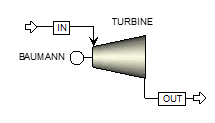
\includegraphics{Content/Appendices/Appendix_F/Figures/AspenPlus_TurbineWetValidation.png}
        \caption{Process flow diagram of the \emph{Aspen Plus v11} simulation used to calculate the performance of a turbine for a wet expansion}
        \label{fig:Aspen_turb_wet_validation}
    \end{figure}

    \begin{listing}[H]
        \caption{Configuration of a turbine performance calculation in \emph{PowerCycle} for saturated steam at temperature \(T\) assuming wet expansion}
        \inputminted[bgcolor=bg,linenos, fontsize=\footnotesize]{python}{Content/Appendices/Appendix_F/Code/TurbineWetPerf_snippet.py}
        \label{lst:PC_turbine_wet_validation}
        \vspace{-20pt}
    \end{listing}

    Assuming the same boundary conditions as the dry expansion case, Section~\ref{sec:PC_dry_turbine_validation}, the calculation results for a wet expansion using \emph{PowerCycle} and \emph{Aspen Plus} can be seen to be in close agreement, with negligible differences, see Table~\ref{table:turbine_wet_validation}.

    \begin{table}[H]
        \caption{The turbine performance calculation results for Aspen Plus v11 and PowerCycle for a wet expansion process}
        \centering 
        \label{table:turbine_wet_validation}
        \begin{tabular}{|p{2.5cm} c c c c|}
    \hline
    \rowcolor{bluepoli!40} % comment this line to remove the color
    \textbf{Parameter} & \textbf{Units} & \textbf{Aspen Plus v11} & \textbf{Power Cycle} & \textbf{Difference/\unit{\percent}} \T\B \\
    \hline \hline
    \(T_{out}\) & \unit{\K} & 318.96 & 318.96 & 0.00 \T\B\\
    \(Q_{out}\) & \unit{\kg\per\kg} & 0.8398 & 0.8398 & 0.00 \T\B\\
    \(\Dot{W}\) & \unit{\kilo\watt} & -591.38 & -591.40 & -0.00 \T\B\\
    \(\Dot{W}_{elec}\) & \unit{\kilo\watt} & -561.81 & -561.83 & -0.00 \T\B\\
    \hline
\end{tabular}
        \\[10pt]
    \end{table}

\section{Pump}
    The inlet stream was initialised to a temperature of \qty{298}{\K} (\qty{25}{\degreeCelsius}) and a pressure of \qty{1}{\bar}. The pump isentropic and motor efficiencies were assumed to be \qty{85}{\percent} and \qty{95}{\percent} respectively. The outlet pressure was set to \qty{10}{\bar}. For a summary of the inlet conditions, see Table~\ref{table:pump_validation_inputs}.

    \begin{table}[H]
        \caption{Comparing the pump performance calculations between PowerCycle and Aspen Plus v11}
        \centering 
        \label{table:pump_validation_inputs}
        \begin{tabular}{|p{2.5cm} c c|}
    \hline
    \rowcolor{bluepoli!40} % comment this line to remove the color
    \textbf{Parameter} & \textbf{Units} & \textbf{Value} \T\B \\
    \hline \hline
    Fluid & - & Water \T\B\\
    \(\Dot{m}\)  & \unit{\kg\per\s} & \num{1} \T\B\\
    \(P_{in}\) & \unit{\bar} & \num{1} \T\B\\
    \(T_{in}\) & \unit{\K} & \num{298} \T\B\\
    \(P_{out}\) & \unit{\bar} & \num{10} \T\B\\
    \hline
\end{tabular}        
        \\[10pt]
    \end{table}

    A standalone pump was modelled in \emph{Aspen Plus}, see Figure~\ref{fig:Aspen_pump_validation}, and \emph{PowerCycle}, see Listing~\ref{lst:PC_pump_validation}. The performance calculation results were found to be in good agreement, Table~\ref{table:pump_validation_outputs}.

    \begin{figure}[H]
        \centering
        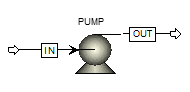
\includegraphics{Content/Appendices/Appendix_F/Figures/AspenPlus_PumpValidation.png}
        \caption{Process flow diagram of the \emph{Aspen Plus v11} simulation used to calculate the performance of a pump}
        \label{fig:Aspen_pump_validation}
    \end{figure}

    \begin{listing}[H]
        \caption{Configuration of a pump performance calculation in \emph{PowerCycle}}
        \inputminted[bgcolor=bg,linenos, fontsize=\footnotesize]{python}{Content/Appendices/Appendix_F/Code/PumpPerf_snippet.py}
        \label{lst:PC_pump_validation}
        \vspace{-20pt}
    \end{listing}

    \begin{table}[H]
        \caption{The pump performance calculation results for \emph{Aspen Plus v11} and \emph{PowerCycle}}
        \centering 
        \label{table:pump_validation_outputs}
        \begin{tabular}{|p{2.5cm} c c c c|}
    \hline
    \rowcolor{bluepoli!40} % comment this line to remove the color
    \textbf{Parameter} & \textbf{Units} & \textbf{Aspen Plus v11} & \textbf{Power Cycle} & \textbf{Difference/\unit{\percent}} \T\B \\
    \hline \hline
    \(T_{out}\) & \unit{\K} & 298.05 & 298.05 & 0.00 \T\B\\
    \(\Dot{W}\) & \unit{\kilo\watt} & 1.06 & 1.06 & 0.02 \T\B\\
    \(\Dot{W}_{elec}\) & \unit{\kilo\watt} & 1.12 & 1.12 & 0.02 \T\B\\
    \hline
\end{tabular}        
        \\[10pt]
    \end{table}

\section{Compressor}
    The inlet stream was initialised to a temperature of \qty{298}{\K} (\qty{25}{\degreeCelsius}) and a pressure of \qty{1}{\bar}. The compressor isentropic and mechnical efficiencies were assumed to be \qty{85}{\percent} and \qty{95}{\percent} respectively. The outlet pressure was set to \qty{10}{\bar}. For a summary of the inlet conditions, see Table~\ref{table:compressor_validation_inputs}.

    \begin{table}[H]
        \caption{Comparison of the compressor performance calculations between \emph{PowerCycle} and \emph{Aspen Plus}}
        \centering 
        \label{table:compressor_validation_inputs}
        \begin{tabular}{|p{2.5cm} c c|}
    \hline
    \rowcolor{bluepoli!40} % comment this line to remove the color
    \textbf{Parameter} & \textbf{Units} & \textbf{Value} \T\B \\
    \hline \hline
    Fluid & - & Water \T\B\\
    \(\Dot{m}\)  & \unit{\kg\per\s} & \num{1} \T\B\\
    \(P_{in}\) & \unit{\bar} & \num{1} \T\B\\
    \(T_{in}\) & \unit{\K} & \num{298} \T\B\\
    \(P_{out}\) & \unit{\bar} & \num{10} \T\B\\
    \hline
\end{tabular}
        \\[10pt]
    \end{table}

    A standalone compressor was modelled in \emph{Aspen Plus v11} and \emph{PowerCycle}, see Figure~\ref{fig:Aspen_comp_validation}, and Listing~\ref{lst:PC_compressor_validation}. The performance calculation results were found to be in good agreement, Table~\ref{table:compressor_validation_outputs}.

    \begin{figure}[H]
        \centering
        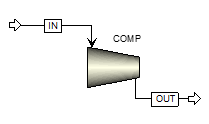
\includegraphics{Content/Appendices/Appendix_F/Figures/AspenPLus_CompValidation.png}
        \caption{Process flow diagram of the \emph{Aspen Plus v11} simulation used to calculate the performance of a pump}
        \label{fig:Aspen_comp_validation}
    \end{figure}

    \begin{listing}[H]
        \caption{Configuration of a compressor performance calculation in \emph{PowerCycle}}
        \inputminted[bgcolor=bg,linenos, fontsize=\footnotesize]{python}{Content/Appendices/Appendix_F/Code/CompressorPerf_snippet.py}
        \label{lst:PC_compressor_validation}
        \vspace{-20pt}
    \end{listing}

    \begin{table}[H]
        \caption{The compressor performance calculation results for \emph{Aspen Plus} and \emph{PowerCycle}}
        \centering 
        \label{table:compressor_validation_outputs}
        \begin{tabular}{|p{2.5cm} c c c c|}
    \hline
    \rowcolor{bluepoli!40} % comment this line to remove the color
    \textbf{Parameter} & \textbf{Units} & \textbf{Aspen Plus v11} & \textbf{Power Cycle} & \textbf{Difference/\unit{\percent}} \T\B \\
    \hline \hline
    \(T_{out}\) & \unit{\K} & 298.05 & 298.05 & 0.00 \T\B\\
    \(\Dot{W}\) & \unit{\kilo\watt} & 1.06 & 1.06 & 0.02 \T\B\\
    \(\Dot{W}_{elec}\) & \unit{\kilo\watt} & 1.12 & 1.12 & 0.02 \T\B\\
    \hline
\end{tabular}
        \\[10pt]
    \end{table}


\section{Multi-Stage Compressor}
    The inlet stream was initialised to a temperature of \qty{298}{\K} (\qty{25}{\degreeCelsius}) and a pressure of \qty{1}{\bar}. The compressor isentropic and mechnical efficiencies were assumed to be \qty{85}{\percent} and \qty{95}{\percent} respectively. The outlet pressure was set to \qty{10}{\bar}. For a summary of the inlet conditions, see Table~\ref{table:multicompressor_validation_inputs}.

    \begin{table}[H]
        \caption{Comparison of the multi-stage compressor performance calculations between \emph{PowerCycle} and \emph{Aspen Plus}}
        \centering 
        \label{table:multicompressor_validation_inputs}
        \begin{tabular}{|p{2.5cm} c c|}
    \hline
    \rowcolor{bluepoli!40} % comment this line to remove the color
    \textbf{Parameter} & \textbf{Units} & \textbf{Value} \T\B \\
    \hline \hline
    Fluid & - & Water \T\B\\
    \(\Dot{m}\)  & \unit{\kg\per\s} & \num{1} \T\B\\
    \(P_{in}\) & \unit{\bar} & \num{1} \T\B\\
    \(T_{in}\) & \unit{\K} & \num{298} \T\B\\
    \(P_{out}\) & \unit{\bar} & \num{10} \T\B\\
    \hline
\end{tabular}
        \\[10pt]
    \end{table}
    
    The multi-stage compressor performance calculations in \emph{Aspen Plus} and \emph{PowerCycle} were compared using corresponding standalone multi-stage compressor models, see Figure~\ref{fig:Aspen_multicomp_validation}, and Listing~\ref{lst:PC_multistage_compressor_validation}. The performance calculation results were found to be in good agreement, Table~\ref{table:multicompressor_validation_outputs}.

    \begin{figure}[H]
        \centering
        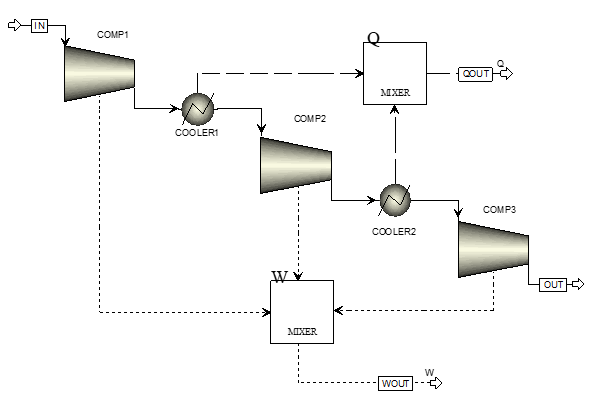
\includegraphics{Content/Appendices/Appendix_F/Figures/AspenPLus_MultiStageCompValidation.png}
        \caption{Process diagram of the \emph{Aspen Plus} simulation used to calculate the performance of a multi-stage compressor}
        \label{fig:Aspen_multicomp_validation}
    \end{figure}

    \begin{listing}[H]
        \caption{Configuration of a multi-stage compressor performance calculation in \emph{PowerCycle}}
        \inputminted[bgcolor=bg,linenos, fontsize=\footnotesize]{python}{Content/Appendices/Appendix_F/Code/MultiStageCompressorPerf_snippet.py}
        \label{lst:PC_multistage_compressor_validation}
        \vspace{-20pt}
    \end{listing}

    \begin{table}[H]
        \caption{The multi-stage compressor performance calculation results for \emph{Aspen Plus v11} and \emph{PowerCycle}}
        \centering 
        \label{table:multicompressor_validation_outputs}
        \begin{tabular}{|p{2.5cm} c c c c|}
    \hline
    \rowcolor{bluepoli!40} % comment this line to remove the color
    \textbf{Parameter} & \textbf{Units} & \textbf{Aspen Plus v11} & \textbf{Power Cycle} & \textbf{Difference/\unit{\percent}} \T\B \\
    \hline \hline
    \(T_{out}\) & \unit{\K} & 298.05 & 298.05 & 0.00 \T\B\\
    \(\Dot{W}\) & \unit{\kilo\watt} & 1.06 & 1.06 & 0.02 \T\B\\
    \(\Dot{W}_{elec}\) & \unit{\kilo\watt} & 1.12 & 1.12 & 0.02 \T\B\\
    \hline
\end{tabular}
        \\[10pt]
    \end{table}
